\documentclass[11pt]{article}
\usepackage[margin=1in]{geometry}
\usepackage{graphicx}
\usepackage{color}
\usepackage{float}
\usepackage{amsmath}
\usepackage{amssymb}
\usepackage{amsthm}
\usepackage{array}
% Import
\usepackage{amsmath,amsthm,graphicx,amssymb,enumerate,longtable,cases,color,natbib,bbm,makecell,accents,subfig,mathtools,endnotes,blkarray,rotating,indentfirst,diagbox,textcomp,authblk,romannum,mathrsfs,tabu,caption,booktabs,array,kantlipsum,xpatch,enumitem,multirow,float}
\geometry{letterpaper} % ... or a4paper or a5paper or ...
\usepackage[percent]{overpic}
\usepackage[singlespacing]{setspace}
\usepackage[bottom]{footmisc}
\usepackage[hidelinks=true]{hyperref}
% \usepackage{setspace}\doublespacing
\usepackage[T1]{fontenc}
\usepackage[utf8]{inputenc}
\usepackage[para,online,flushleft]{threeparttable}
\usepackage[all]{xy}
\newcommand{\rowgroup}[1]{\hspace{-1em}#1}
\newcommand{\E}{\mathbb{E}}
\newcommand{\halfspace}{\hspace{0.2mm}}
\newcommand{\AM}{{\tiny\hspace{-0.7mm} AM \hspace{0.7mm}}}
\newcommand{\PM}{{\tiny\hspace{-0.7mm} PM \hspace{0.7mm}}}
\newcommand{\Wedgesmall}{\text{{\small$\wedge$}}}
\newcommand{\Wedgefootnotesize}{\text{{\footnotesize$\wedge$}}}
\newcommand{\Wedgescriptsize}{\text{{\scriptsize$\wedge$}}}
\newcommand{\BSmall}[1]{\mkern-1.7mu\raisebox{-1.2pt}{\scalebox{0.9}{$\scriptscriptstyle B$}}}
\newcommand{\NSmall}[1]{\mkern-1.7mu\raisebox{-1.2pt}{\scalebox{0.9}{$\scriptscriptstyle N$}}}
\newcommand{\Dispatch}[1]{{#1}}
\newcommand{\Relocation}[1]{\tilde{#1}}
\newcommand{\Plus}{\raisebox{.4\height}{\scalebox{.6}{+}}}
\newcommand{\Minus}{\raisebox{.4\height}{\scalebox{.8}{-}}}
\def\minus{\texttt{-}}
\newcommand*\rot{\rotatebox{90}}
\newcommand{\nquad}{\kern-1em}
\DeclareRobustCommand{\rchi}{{\mathpalette\irchi\relax}}
\newcommand{\irchi}[2]{\raisebox{\depth}{$#1\chi$}} % inner command, used by \rchi
\newlength{\dhatheight}
\newcommand{\doublehat}[1]{%
	\settoheight{\dhatheight}{\ensuremath{\hat{#1}}}%
	\addtolength{\dhatheight}{-0.35ex}\hat{\vphantom{\rule{1pt}{\dhatheight}}\smash{\hat{#1}}}}

% \makeatletter
% \newcommand{\Rom}[1]{\expandafter\@slowromancap\romannumeral #1@}
% \newcommand{\Biggg}{\bBigg@{2.5}}
% \newcommand{\vast}{\bBigg@{3}}
% \newcommand{\Vast}{\bBigg@{3.5}}
% \newcommand{\massive}{\bBigg@{4.5}}
% \newcommand{\Massive}{\bBigg@{6}}
% \renewcommand\subparagraph{%
% 	\@startsection {subparagraph}{5}{\z@ }{3.25ex \@plus 1ex
% 		\@minus .2ex}{-1em}{\normalfont \normalsize \bfseries }}%
% \newcommand\notsotiny{\@setfontsize\notsotiny\@vipt\@viipt}
% \newcommand{\thickhline}{%
% 	\noalign {\ifnum 0=`}\fi \hrule height 1pt
% 	\futurelet \reserved@a \@xhline}
% \newcolumntype{"}{@{\hskip\tabcolsep\vrule width 1pt\hskip\tabcolsep}}
% \newcommand{\Blue}[1]{\textcolor{blue}{#1}}
% \newcommand{\Red}[1]{\textcolor{red}{#1}}
% \newcommand{\Purple}[1]{\textcolor{purple}{#1}}
% \newcommand{\Grey}[1]{\textcolor{gray}{#1}}
% \newcommand{\Orange}[1]{\textcolor{orange}{#1}}
\newcommand{\overbar}[1]{\mkern 1.5mu\overline{\mkern-1.5mu#1\mkern-1.5mu}\mkern 1.5mu}
\newcommand{\PreserveBackslash}[1]{\let\temp=\\#1\let\\=\temp}
\newcolumntype{C}[1]{>{\PreserveBackslash\centering}p{#1}}
\newcolumntype{R}[1]{>{\PreserveBackslash\raggedleft}p{#1}}
\newcolumntype{L}[1]{>{\PreserveBackslash\raggedright}p{#1}}
% End Import
\DeclareMathOperator*{\argmin}{argmin}
\DeclareMathOperator*{\argmax}{argmax}
\newtheoremstyle{ModifiedStyle}
{\topsep} % Space above
{3pt} % Space below
{} % Body font
{} % Indent amount
{\bfseries} % Theorem head font
{.} % Punctuation after theorem head
{.5em} % Space after theorem head
{} % Theorem head spec (can be left empty, meaning 'normal')
\theoremstyle{ModifiedStyle}
\newtheorem{remark}{Remark}
\newtheorem{assumption}{Assumption}
\usepackage[
    backend=biber,
    style=authoryear,
  ]{biblatex}

\addbibresource{main.bib}

\pagenumbering{arabic}

\title{Simulation Study Overview}
\author{}

\begin{document}
\maketitle
\tableofcontents

% \section{Introduction}
%   One of the chief criticisms of the US criminal justice system is that many states in the US exhibit large regional variation in sentencing. This means that given the same crime, the probability of incarceration and the length of sentence vary considerably from county to county. To reduce variability in sentencing, many states (e.g. Florida, Minnesota, Washington) have introduced sentencing guidelines. These guidelines generally reduce the amount of discretion a judge has when deciding the length of a sentence. \cite{hester2012criminal} found that South Carolina has less county-level variation in sentencing than many states with sentencing guidelines.
%
%   A follow up study (\cite{hester2017conditional}) suggests that this might be due to the practice of judge rotation in South Carolina.
%   Judges in South Carolina don't sit exclusively in one county. Instead, they split their time amongst several counties in the state. For reference, the average judge hears cases in 12 counties throughout the year. Defendants are given some choice with regards to the date their case will be heard. Furthermore, defendants are made aware of which judges will be sitting in which counties in the near future. This gives them the ability to "shop" for judges, although subject to some constraints (e.g. judge availability).
%
%   The goal of this project is study how some system features affect sentencing outcomes. The system features we focus on are judge capacity and defendant choice. The outcomes we focus on are across county variation in sentencing and backlog of defendants. We study the system through simulation. We estimate relevant parameters using a rich dataset of sentencing data from South Carolina. The model we simulate builds on the work of \cite{wang2019}.

\section{Data}
  We have two main data sources: sentencing data and judge schedules, both of them are for the 2001 fiscal year. We obtained the data from the authors of \cite{hester2017conditional}. We briefly describe both datasets below.

  \subsection{Sentencing Data}
    The sentencing data contains information about 17,671 sentencing events in South Carolina from August 2000-July 2001. Each sentencing event contains an identifier for the judge who heard the case, the county the case was heard in, categorical variables describing the offense, and some defendant characteristics (e.g. race, age, and criminal history). There are 50 judges and 46 counties in the dataset. A full list of the variables we use can be found in Table \ref{sent-vars}.

    \begin{table}[H]
      \caption{Sentencing Data Variables}
      \label{sent-vars}
      \begin{tabular}{|l|l|}
\hline
\textbf{Variable} & \textbf{Description}                                             \\ \hline
date              & date of sentence                                                 \\ \hline
county            & county where the sentence was decided                            \\ \hline
circuit           & circuit court where sentence was decided                         \\ \hline
judge             & numerical identifier for the judge who head the case             \\ \hline
trial             & binary variable indicating whether the case went to trial        \\ \hline
incarc         & binary variable indicating whether the sentence includes incarceration                \\ \hline
statute           & the code of law that the offender broke (e.g. 56-05-0750(B)(1))  \\ \hline
offdescr          & a description of the offense (e.g. driving under the influence)  \\ \hline
counts            & numerical variable                                               \\ \hline
statute\_first & the code of law that the offender broke, identical to 'statute' variable              \\ \hline
offdescr\_first   & a description of the first offense, similar to offdescr          \\ \hline
offtyped       & detailed categorical offense type, there are 10 values (rape, assault,   theft, etc). \\ \hline
sgc\_offcode   & a numerical code that is used to determine the minimum sentence   multiplier          \\ \hline
offtypeLibHyp     & categorical offense type (property, violent, drug, other)        \\ \hline
offser            & offense seriousness, ranges from 1-8                             \\ \hline
ccpnts            & numeric values between 1 and 68                                  \\ \hline
ccpts99           & commitment score, an alternative measure of offense seriousness. \\ \hline
crimhist          & defendant criminal history, takes 5 categorical values           \\ \hline
ppoints           & numerical values between 0-1014                                  \\ \hline
male              & binary variable indicating sex                                   \\ \hline
age               & age of defendant at sentencing, ranges 15-81                     \\ \hline
black             & binary variable indicating whether defendant is black            \\ \hline
sentence          & length of sentence in months, ranges 0-11988                     \\ \hline
expmin            & expected minimum sentence                                        \\ \hline
\end{tabular}

    \end{table}

    \subsubsection{Sample}
      In the raw data, there are 51 distinct judge ID's. However, according to \cite{hester2017conditional}, judge 1 is a combination of several judges that had few sentencing events. As a result, we exclude judge 1 from our sample, which leaves us with 17,516 observations.

    \subsubsection{Imputation of Missing Dates}
      After removing the sentencing events heard by Judge 1, there are 1,482 sentencing events with the \textit{date} field missing. This is the only variable with missing values in the entire dataset. We impute the dates for these events in the following way. Recall that the judge name and county are still available for sentencing events with missing dates. In general, when imputing the dates for sentencing events with missing dates, we first use the master calendar to determine a set of possible dates in which the sentencing event could have occurred, and then we assign the events with missing dates as evenly as possible across these possible dates. So, for example, if there are 5 sentencing events with missing dates and 4 potential dates, then each of the potential dates would get assigned a sentencing event, and the first of the potential dates would get the remaining one.
      Suppose that judge $j$ has $m$ sentencing events with missing dates in county $c$ (which is in circuit $k$). The set of potential dates we would assign these sentencing events to would evolve in the following way. In each category, the days are ordered from earliest to latest.

      \begin{enumerate}
        \item \textbf{Matching county, GS:} Days in the master calendar in which judge $j$ had a "GS" assignment to county $c$.
        \item \textbf{Matching county, non-GS:} Days in the master calendar in which judge $j$ had a non-"GS" assignment to county $c$.
        \item \textbf{Matching circuit, GS:} Days in the master calendar in which judge $j$ had a "GS" assignment to a county in circuit $k$.
        \item \textbf{Matching circuit, non-GS:} Days in the master calendar in which judge $j$ had a non-"GS" assignment to a county in circuit $k$.
        \item \textbf{Sentencing data match:} Days in which we observe sentencing events in the sentencing data for judge $j$ in county $c$.
        \item \textbf{Any day, GS:} Days in the master calendar in which judge $j$ had a "GS" assignment to any county.
      \end{enumerate}

      So, first, we would try to assign the sentencing events to days in the first set, if that set is empty, we would move on to the next set until we found a non-empty set. Using this method, we are able to impute the missing dates for all sentencing events with missing dates. Table \ref{tab:imp} contains the distribution of the imputation method used for pleas with missing dates.

      \begin{table}[H]
          \centering
          \caption{Distribution of missing events}
          \label{tab:imp}
          \begin{tabular}{|l|l|}
          \hline
          \textbf{Imputation Group}   & \textbf{Share of Pleas} \\ \hline
          1. Matching county, GS      & 0.825                   \\ \hline
          2. Matching county, non-GS  & 0.024                   \\ \hline
          3. Matching circuit, GS     & 0.02                    \\ \hline
          4. Matching circuit, non-GS & 0.006                   \\ \hline
          4. Sentencing data match & 0.026 \\ \hline
          5. Any day, GS              & 0.098                    \\ \hline
          \end{tabular}
      \end{table}

  \subsection{Master Calendar Data}
    This dataset contains information about each judge's assignment for each week of the fiscal year 2001. A snapshot of the calendar can be seen in figure \ref{fig-calendar}. Each assignment generally contains the county each judge was assigned to and the assignment type. The assignment type refers to the kind of cases a judge is scheduled to hear (civil or criminal).
    \begin{figure}[h]
        \centering
        \caption{Snapshot of Judge Calendar}
        \label{fig-calendar}
        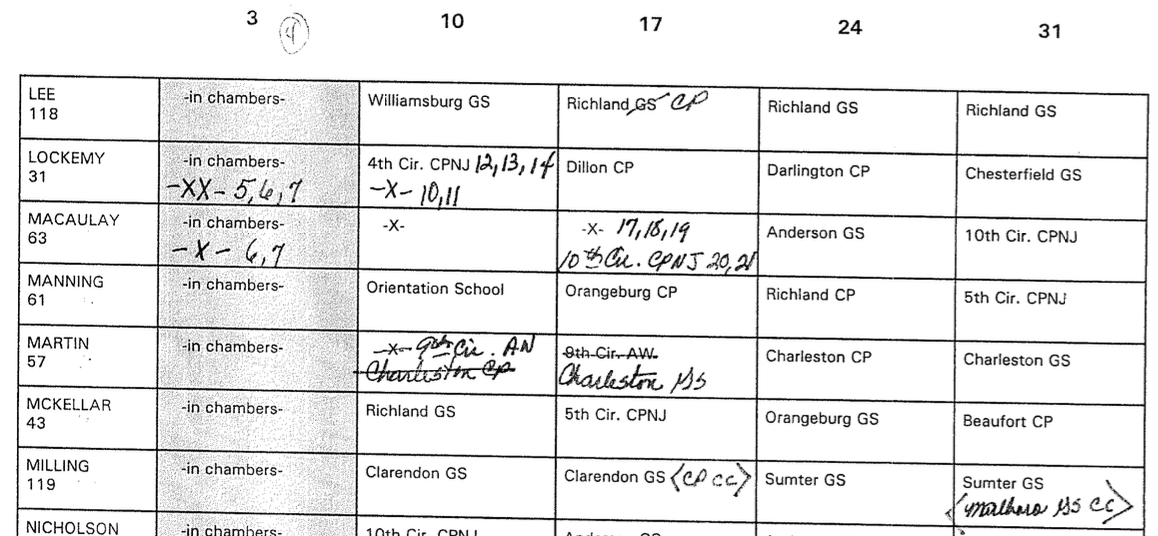
\includegraphics[width=0.75\textwidth, keepaspectratio=true]{Figures/Fig4.png}
      \end{figure}

    \subsection{Assignments}
      The judges were generally assigned to either specific counties or to circuit courts. In the master calendar data, $75\%$ of all judge assignments were to either a specific county or to a circuit court. The remaining assignments were to one of the categories in Table \ref{tab-special-assignments}. As can be seen, outside of "in chambers" they generally pertain to special circumstances.

      \begin{table}[H]
        \centering
        \caption{Non county or circuit court assignments}
        \label{tab-special-assignments}
        \begin{tabular}{l}
        \hline
        \textbf{Assignment}                      \\ \hline
        In chambers        \\
        Orientation School \\
        Medical            \\
        Family Death       \\
        Sick              \\
        Military           \\
        X                  \\ \hline
        \end{tabular}
      \end{table}

    \subsubsection{Assignment Types}
      Judge calendar assignments generally have an acronym indicating the type of the assignment (e.g. Marion GS). There are eight different assignment types, each with a corresponding acronym. Assignments can have more than one type (e.g. Marion GS CC). Our study focuses on criminal cases, which are heard in general sessions (GS). Some assignment types, like CP (common pleas), are for civil cases. A full list of the assignment type acronyms and their meanings can be found in Table \ref{tab-assignment-types}.

      \begin{table}[H]
        \centering
        \caption{Assignment Type Acronyms. The share column specifies the share of all assignments that include that assignment type.}
        \label{tab-assignment-types}
        \begin{tabular}{L{20mm}L{50mm}L{20mm}}
  \hline
  Acronym & Meaning & Share \\
  \hline
  %\rowgroup{Consumer Surplus} \\
  GS & General Session & 0.36 \\
  CC & Circuit Court & 0.02\\
  SGJ & State Grand Jury & 0.01\\
  CP & Common Pleas & 0.26 \\
  CPNJ & Common Pleas Non-Jury & 0.13 \\
  PCR & Post Conviction Relief & 0.03  \\
  Capital PCR & Capital Post Conviction Relief & < 0.01 \\
  AW & Administrative Week & 0.01 \\
  \hline
\end{tabular}

      \end{table}

			% Assignments of type GS are exclusively for criminal cases. Common pleas refers to civil cases. TODO: Elaborate on the description of each of these categories. Especially GS.

    \subsubsection{Parsing}
      As can be seen from Figure \ref{fig-calendar}, the assignments in the raw calendar data are on a weekly basis. However, several parts of our analysis stood to benefit from having the daily assignments for each judge, as opposed to only the weekly assignment. For example, this allowed us to more accurately count the total number of days a judge was assigned to a county, or to more accurately determine if there was discrepancy between the sentencing data and the calendar data. The goal of the parsing was to turn the weekly assignemnts in the calendar data into daily assignments. In other words, we wanted to determine where each judge \textit{should have been} each day of the year (according to the calendar data). The end goal of the parsing is to create a dataset that contains at least one observation for each judge's location in each day of the year. This dataset will represent where the judge should have been according to the calendar data.

      A judge can be assigned to one or multiple counties in a week, and we observe 5 different kinds of assignments: single assignment, single assignment with dates, multiple assignment, multiple assignment with some dates, and multiple assignment with all dates. We parse the calendar data to determine each judge's schedule for every day of the year. In the resulting data, the unit of observation is judge, day, county. Note that the only potentially ambiguous assignment types are multiple assignment and multiple assignment with some dates. By ambiguous, we mean that the calendar data does not specify a unique location for a judge. For example, in the single assignment case the judge is only supposed to be in one county (according to the calendar data). However, in the multiple assignment case, it is not clear in which county the judge should be (according to the calendar data). For these ambiguous assignment types, we set the judge to be in all counties that he is scheduled to be in. One portion of our analysis involves counting the number of days that a judge was assigned to a specific county. For days in which a judge is assigned to multiple counties, we normalize the number of days he/she is assigned to each county so that the sum of the assignments for each day is equal to one. For example, if judge 2 is scheduled for both Marion and Horry in the week of March 19-March 23, for each day of that week our data would include an observation for judge 2 in Horry and an observation for judge 2 in Marion. Furthermore, for each of these days we would say that judge 2 was assigned to 0.5 days in Horry and 0.5 days in Marion. An example of what our parsed data looks like can be seen in table \ref{tab-calendar-example}.

      \begin{table}[H]
        \centering
        \caption{Assignment Types}
        \label{tab-assignments}
        \begin{tabular}{|l|l|}
\hline
\textbf{Assignment} & \textbf{Example}                \\ \hline
Single              & Marion                          \\ \hline
Single with dates   & Marion 23, 24, 25               \\ \hline
Multiple            & Marion, Horry                   \\ \hline
Multiple some dates & Marion 23, 24, Horry            \\ \hline
Multiple all dates  & Marion 23, 24, Horry 25, 26, 27 \\ \hline
\end{tabular}

      \end{table}

      \begin{table}[H]
        \centering
        \caption{Example of Parsed Calendar Data, here Judge 3 is scheduled for both Horry and Greenville on March 19.}
        \label{tab-calendar-example}
        
\begin{tabular}{|l|l|l|l|}
\hline
\textbf{Judge} & \textbf{Day} & \textbf{County} & \textbf{Days Assigned} \\ \hline
2              & 2001-03-19   & Marion          & 1 \\ \hline
3              & 2001-03-19   & Horry           & 0.5 \\ \hline
3              & 2001-03-19   & Greenville      & 0.5\\ \hline
\end{tabular}

      \end{table}

  \subsection{Merging the Sentencing Data and the Calendar Data}
	  \label{mapping-judge-names}
    The main challenge in using the two datasets is that they don't share a common identifier for judges. The sentencing data uses numerical IDs to
    identify judges, while the calendar data uses judge names to identify them. There is no mapping from judge numbers to judge names in the raw data. To map judge ID's to judge names, we assign each Judge ID to the judge name in the schedule data whose schedule overlaps the most with that Judge ID. We consider the sentencing data and schedule data to overlap for a Judge ID and a Judge name in a specific week if the Judge ID in consideration has a sentencing event in a county that that judge name is assigned to in that week. So, if in Week 12 judge 'John Doe' is assigned to 'Aitken' county, and we see a sentencing event for Judge ID $n$ in 'Aitken' county on Week 12, we would consider their schedules to be overlapping in that week. Assigning each judge ID to the judge name with the most overlap yields a unique mapping (i.e. there are never any ties). We also tried two other methods, and they yielded the same results. The two other methods as well as the final mapping can be found in Appendix \ref{app-map}.

\section{Model}
  We build on the model developed by \cite{wang2019}. There are three agents: the judge, the defendant, and the prosecutor. The prosecutor proposes a plea offer, and the judge and the defendant choose whether to accept. The game evolves in the following steps:

  \begin{enumerate}
    \item The defendant chooses the judge/decides when to go to court
    \item The prosecutor makes a plea offer
    \item The defendant decides whether to accept the plea offer or go to trial
  \end{enumerate}

  Each defendant is characterized by the following quantities: $\theta$ - the probability of conviction at trial, and $\tau$ - the expected sentence length if convicted in trial. Each defendant additionally has an idiosyncratic cost of going to trial, $c_d >0$ (we relax this assumption later). A defendant will accept a plea offer, $s$, if $s \leq \theta \tau + c_d$.\\

  Judges are modeled by their harshness, $h$. Given a defendant, $\theta \tau$ and a plea offer, $s$, the lowest plea offer the judge will accept is denoted by $l_j(\theta \tau)$ and the maximum plea offer the judge will accept is denoted by $u_j(\theta \tau)$.\\

  As a result, given a specific judge $j$, the optimal sentence for the prosecutor to offer is $s^* = \min(\theta \tau + c_d,u_j(\theta \tau))$. This quantity is also the defendant's cost. Finally, the case goes to trial if $\theta \tau + c_d < l_j(\theta \tau)$.

\section{Estimation}
  For the simulation, we have to estimate several of the model's parameters. In this section, we provide a detailed description of how we estimate each parameter, including the sample used.

  \subsection{Assumptions/Restrictions}
    \begin{table}[H]
      \centering
      \caption{Assumptions/Restrictions Used}
      \label{tab:assumptions}
      \begin{tabular}{ll}
      \hline
      \textbf{Assumption/Restriction}                              & \textbf{Section Used}        \\ \hline
      We only use the trial sentencing events to estimate $\theta$ & \ref{theta-estimation}       \\
      We only use the trial sentencing events to estimate $\tau$   & \ref{tau-estimation}         \\
      We currently only use a subset of the data to estimate $c_d$ & \ref{c_d-estimation}         \\
      We add the point $(0,0)$ to the convex hull of every judge   & \ref{convex_hull-estimation} \\
      We assume (TBD) when using regression model & \ref{service_rate-estimation}} \\ \hline
      \end{tabular}
    \end{table}

  \subsection{Probability of Conviction at Trial - $\theta$}
    \label{theta-estimation}
    We currently estimate this using $l_2$ regularized logistic regression with a penalty parameter of 1. We use the following variables to predict this quantity: Black, Offense Type, and Offense Seriousness. We represent all variables as binary variables. We split our sample into train and test sets using a 75/25 split to evaluate the performance of our classifier. Our classifier's performance can be seen in table \ref{classifier-performance}. The classifier outputs prediction probabilities, which is what we use for $\theta$. The classifier's prediction probability can be interpreted as the probability that the observation will have a value of 1 for the incarceration variable. The final classifier we use to predict $\theta$ for all observations in our dataset is trained on the full training set.

    \begin{table}[H]
      \centering
      \caption{Evaluation Metrics for Classifier}
      \label{classifier-performance}
      \begin{tabular}{|l|l|}
      \hline
      \textbf{Metric} & \textbf{Score} \\ \hline
      AUC             & 0.93           \\ \hline
      F1              & 0.94           \\ \hline
      Accuracy        & 0.89           \\ \hline
      \end{tabular}
    \end{table}

    \subsubsection{Sample}
      We only use the observations in the data that are trials and that have non missing values for the predictor variables. There are only 256 observations in the data meeting this criteria. Of these 256 observations, 247 resulted in a conviction.

    \subsubsection{Proposed Changes}
      We should consider jointly estimating $\theta$ and $\tau$ using a Hurdle Regression model as in Hester and Hartman 2017.

  \subsection{Expected Sentence Length if Convicted - $\tau$}
    \label{tau-estimation}
    We currently estimate this using Negative Binomial Regression. We use the Cameron-Trivedi test for overdispersion to choose the overdispersion parameter. As in Hester and Hartman 2017, our dependent variable is the expected minimum sentence. We use the following variables to predict this quantity: Black, Age, Offense Type, and Offense Seriousness.

    \subsubsection{Sample}
      We only use the observations in the data that are trials and that have non missing values for the predictor variables. There are only 256 observations in the data meeting this criteria.

    \subsubsection{Proposed Changes}
      We should consider jointly estimating $\theta$ and $\tau$ using a Hurdle Regression model as in Hester and Hartman 2017.

  \subsection{Defendant Cost of Trial - $c_d$}
    \label{c_d-estimation}
    We are currently estimating this using only the first method described in the Write-Up. In this method, we use the subset of cases where the sentence, $s$, is less than $u_j(\theta \tau)$. In these cases, our model implies that $c_d = s - \theta \tau$.

    \subsubsection{Proposed Changes}
      We should implement the maximum likelihood estimation procedure described in Nasser's document for the other cases. Here's the discussion:
      Recall that $i=1,\ldots,I_j$ are the plea bargains judge $j$ oversaw, and that their sentence is given by $s_i=\min(\theta_i\tau_i+c_d(i),u_i)$, where $u_i = u_j(\theta_i\tau_i)$ and $u_j(\cdot)$ is defined above. We define the sets $\mathcal{I}_j^1$ and $\mathcal{I}_j^2$ as follows:
  			\begin{align*}
  				\mathcal{I}_j^1 &\,=\, \{i=1,\ldots,I_j: s < u_i\}, \\
  				\mathcal{I}_j^2 &\,=\, \{1,\ldots,I_j\} \,\backslash\, \mathcal{I}_j^1 \,=\, \{i=1,\ldots,I_j:s_i=u_i\}.
  			\end{align*}
  			Then, we can infer $c_d(i) = s_i - \hat{\theta}_i\hat{\tau}_i$ for $i\in\mathcal{I}_j^1$. On the other hand, we can only infer that $c_d(i) \geq u_i - \hat{\theta}_i\hat{\tau}_i$ for $i\in\mathcal{I}^2_j$.

  		Next, we let $K_j$ denote the number of trials judge $j$ oversaw, which are indexed by $k \in \mathcal{K}_j = \{1,\ldots,K_j\}$. Recall that a case goes to trial if $\theta_i\tau_i+c_d(i)<l_i$. Thus, for $i=1,\ldots,K_j$, we infer that $c_d(i) < l_i-\hat{\theta}_i\hat{\tau}_i$.

  		In summary, although we can impute $c_d(i)$ exactly for $i\in\mathcal{I}_j^1$, we can only infer that $c_d(i)$ falls into an interval for $i\in\mathcal{I}^2_j\cup \mathcal{K}_j$. However, assuming a parametric distribution for $c_d$, e.g., $c_d \sim N(\mu,\sigma^2)$, we can estimate its parameters using maximum likelihood. To this end, we let $F$ and $f$ denote the cdf and pdf of the distribution of $c_d$, and define the likelihood function $\mathscr{L}_j$ as follows:
  		\begin{align*}
  			\mathscr{L}_j \,=\, \prod_{i\in\mathcal{I}_j^1} f(s_i-\hat{\theta}_i\hat{\tau}_i) \prod_{i\in\mathcal{I}_j^2} \bar{F}(u_i-\hat{\theta}_i\hat{\tau}_i) \prod_{i\in \mathcal{K}_j} F(l_i-\hat{\theta}_i\hat{\tau}_i).
  		\end{align*}
  		Then, we let $\mathscr{L} = \prod_{j=1}^J \mathscr{L}_j$ and $\argmax \mathscr{L}$ helps us choose the parameters of the distribution $F$.
  		\begin{remark}
  			Note that the approach proposed immediately above allows $c_d$ to be negative. We can attribute this to $c_d(i)$ being the cost of trial plus an idiosyncratic shock specific to defendant $i$, which encompasses all factors that are not captured explicitly in the model.
  		\end{remark}
  		\begin{remark}
  			We envision drawing defendant profiles (along with their cases) with replacement from the dataset at a particular weekly rate in our simulation study. As we do so, we can set $c_d = c_d(i)$ whenever we draw a defendant who falls into the set $\mathcal{I}_j^1$ for some judge $j$. Otherwise, we can consider the following two cases:
  			\begin{itemize}
  				\vspace{-2mm}
  				\item[] \hspace{-10mm}\textbf{Case i)} Defendant $i$ is in the set $\mathcal{I}_j^2$ for some judge $j$. Then, we draw $c_d(i)$ from the conditional distribution $F(x|x\geq u_j-\hat{\theta}_i\hat{\tau}_i)$.
  				\vspace{-2mm}
  				\item[] \hspace{-10mm}\textbf{Case ii)} Defendant $i$ is in the set $K_j$ for some judge $j$. Then, we draw $c_d(i)$ from the conditional distribution $F(x|x\leq l_j-\hat{\theta}_i\hat{\tau}_i)$.
  			\end{itemize}
  		\end{remark}

  \subsection{Judge maximum and minimum plea - $l_j(\theta \tau),u_j(\theta \tau)$}\label{convex_hull-estimation}
    \paragraph{Mathematical Description} Recall that a key quantity for us is $\theta\tau$. Fix a judge, say judge $j$, and focus only on the pleas he sentenced. For each such case, we can calculate $\hat{\theta}\hat{\tau}$ using the estimates from the hurdle model described in Section (tbd). Suppose judge $j$ handled $I_j$ such cases, indexed by $i=1,\ldots,I_j$. Let $\mathcal{A}_j$ denote the convex hull of the origin $(0,0)$ and the points $(\hat{\theta}_i\hat{\tau}_i,s_i)$ for $i=1,\ldots,I_j$. Given the set $\mathcal{A}_j$, we impute $l_j(\cdot)$ and $u_j(\cdot)$ as functions of $\theta\tau$ as follows:
		\begin{align*}
			&l_j(\theta\tau) \,=\, \min\{y:(\theta\tau,y)\in\mathcal{A}_j \} \\
			&u_j(\theta\tau) \,=\, \max\{y:(\theta\tau,y)\in\mathcal{A}_j \}
		\end{align*}

   \paragraph{Implementation}
   Suppose we have the simplices of the convex hull for a specific judge, and that they are given as tuples of two points $((x_1,y_1),(x_2,y_2))$. Given a specific $\theta \tau$ we implement the convex hull approach by iterating over the simplices of the convex hull, and finding the two simplices on which $\theta \tau$ lies. In other words, we find the two line segments on the boundary of the convex hull whose domain includes $\theta \tau$. We then find the value of the convex hull boundary at $\theta \tau$ in each of these two line segments using linear interpolation. The largest (smallest) of these two values is $u_j (l_j)$. In cases where $\theta_1 \tau_1$ is not in the domain of the convex hull because it is too large, we use the largest value in the convex hull to find $u_j (l_j)$. $\theta_1 \tau_1$ will never be too small because all convex hulls include $(0,0)$ and $\theta_1 \tau_1 \geq 0$. Figure \ref{fig-convex-hull} contains an illustration:

	 \textbf{Note:} we should think about what to do in cases where $\theta_1 \tau_1$ is not in the convex hull. Figure \ref{fig-convex-hull} contains an illustration:

    \begin{figure}[H]
      \centering
      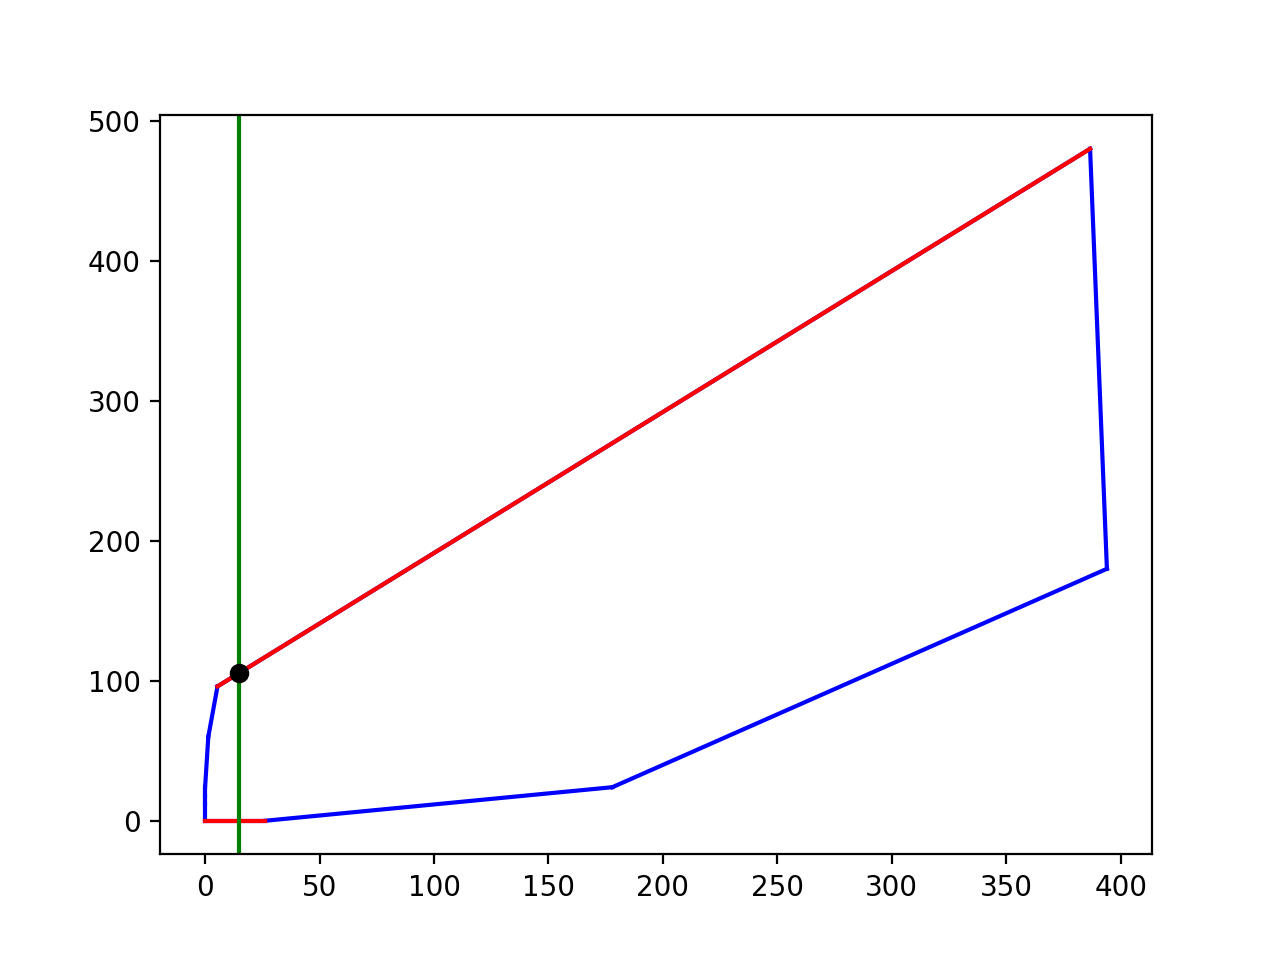
\includegraphics[width=0.65\textwidth]{../../output/figures/Exploration/convex_hull_max.png}
      \caption{Example of convex hull approach. The convex hull is in blue, the two line segments containing $\theta \tau$ are in red, and the green line intercepts the x-axis at $\theta \tau$. The black dot would be the maximum plea.}
      \label{fig-convex-hull}
    \end{figure}

    \subsubsection{Sample}
      Here, to estimate $l_j(\theta \tau),u_j(\theta \tau)$ for a specific judge, $j$, we use all of pleas judge $j$ heard. In other words, we exclude all of $j$'s trials. We also add the point $(0,0)$ to the convex hull of every judge.

  \subsection{County Arrival Rates - $\lambda_c$}
    \label{lambda_c-estimation}
    We set each county's arrival rate to be equal to the average number of sentencing events per week in that county, as observed in the data. Let $N_{cw}$ denote the number of sentencing events in county $c$ in week $w$, county $c$'s arrival rate is defined as: $\lambda_c = \frac{\sum_w N_{cw}}{\sum_w 1}$. We are currently using all pleas and all weeks in our data to calculate this.

  \subsection{Service Rates - $\mu_p,\mu_t$}
    \label{service_rate-estimation}
    \subsubsection{Samples}
      \paragraph{Plea MLE Sample} This is the sample we use for the maximum likelihood estimation part of the ad-hoc algorithm. We also refer to this sample as "clean days". For this, we only consider pleas that happened on days which satisfy the following conditions:
        \begin{table}[H]
          \centering
          \caption{MLE Plea Sample Exclusion Criteria}
          \begin{tabular}{|l|}
          \hline
          \textbf{Condition}                                                  \\ \hline
          No inconsistencies between sentencing data and calendar \\ \hline
          Judge has at least 10 'clean' days                      \\ \hline
          Judge has at least one sentencing event that day         \\ \hline
          Judge is only assigned to one county that day          \\ \hline
          Judge only sentences in one county that day             \\ \hline
          Judge never has more than 35 sentencing events in this county \\ \hline
          Judge calendar assignment is of type "GS"           \\ \hline
          \end{tabular}
        \end{table}
      % \textbf{Sensitivity Analysis:} Add these one by one, similar to how controls are presented in Econ papers, and see how the quantity of interest changes as they are added. We could also add them in groups. Some of these correspond to outlier control and others to day cleanliness. We can run it with and without each group.

      \paragraph{Plea Arrival Rate Sample} This is the sample we use to estimate the plea arrival rate, $\theta$ in the ad-hoc algorithm. The calculation of $\theta$ involves two quantities: the total number of pleas in the data, $N_p$, and $d$, the total number of judge days. $d$ is meant to represent the number of days in which a judge could have been working on pleas. As a result, for $d$ we include all days of type "GS", and we include days of other work types in which we observe sentencing events. $N_p$ currently includes all pleas in our data.

      \paragraph{Trial Rate Sample} This is the sample we use to estimate the trial service rate, $\mu_t$. When calculating the total number of days a judge was assigned to a county, we include all days he had a "GS" assignment to that county in the master calendar, and all days of type non-GS in which we observe a sentencing event. Note, this is the same criteria as used above for the plea arrival rate sample. We include all pleas and all trials when calculating the total number of pleas and trials the judge heard in that county. We focus on the judge-county combinations that satisfy the following conditions:

        \begin{table}[H]
        \centering
        \caption{Trial Service Rate Exclusion Criteria}
        \begin{tabular}{|l|}
        \hline
        \textbf{Condition}                                                       \\ \hline
        Judge never has more than 35 sentencing events in one day in this county \\
        Judge has at least 2 trial in this county                                \\ \hline
        \end{tabular}
        \end{table}

        % \textbf{Proposed Changes:} Since our explicit assumption is that judges only spend time on pleas or trials when calculating the expected trial days and expected plea days, I think it might make sense to exclude days where it is unlikely that the judge was working on either of those two tasks, like when they are hearing civil cases. \textbf{Sensitivity Analysis:} We can think of our conditions as corresponding to day cleanliness and outlier control, and group them based on those criteria. We can then add them by group and see how our estimate evolves. If any criteria significantly changes the estimate, we should argue why it is a good criteria to have.

    \subsubsection{Estimation of $\mu_t$}
      \label{mu_t-estimation}
      To estimate the trial service rate, we focus on the judge-county combinations that satisfy the conditions described in the Trial Rate Sample paragraph. Let $K$ denote the number judge-county combinations satisfying these two conditions. We number these judge-county combinations $1,\ldots,K$ and define $\mathcal{K} = \{1,\ldots,K\}$. For judge-county $k \in \mathcal{K}$, we let $n_p(k)$ and $n_t(k)$ denote the total number of pleas and the total number of trials undertaken by this judge in this county. Similarly, for judge-county $k \in \mathcal{K}$, we let $T(k)$ denote the number of days this judge was assigned to this county.\footnote{In calculating $T(k)$ for $k\in\mathcal{K}$, we assume the judge divides his time equally among the county assignments to which he is assigned if he is assigned to multiple counties on a day.}

			First, we assume the judges in judge-county combinations $k\in\mathcal{K}$ never idle. If this assumption was correct, the trial service rate of judge-county $k\in\mathcal{K}$ would be
			\begin{align*}
				\hat{\mu}_t(k) \,=\, \frac{n_t(k)}{T(k) - n_p(k) / \hat{\mu}_p}.
			\end{align*}

      The tuples $(n_t(k),{\hat{\mu}_t(k)})$ for $k\in\mathcal{K}$ are depicted in Figure \ref{Figure_Trial_Sercice_Rate_Vs_Trial_Per_County}.
			%
			\begin{figure}[H]
				\centering
				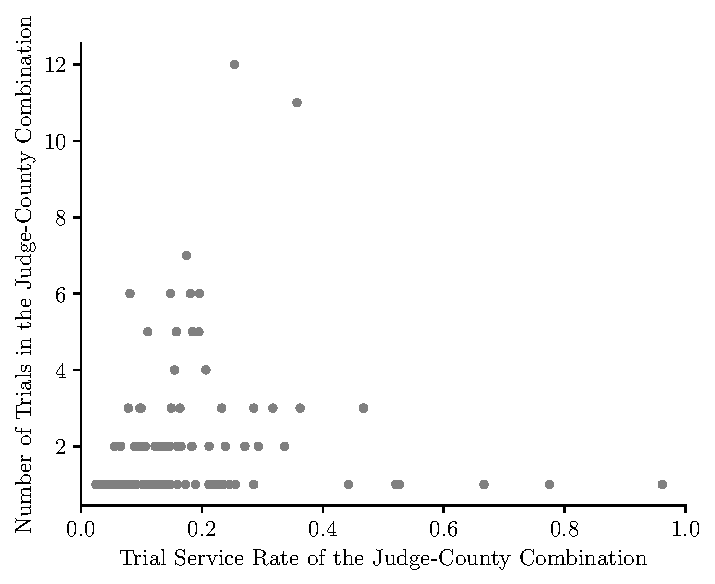
\includegraphics[scale=0.75]{Figures/Judge_Capacity_Vs_Number_of_Trials}
				\vspace{-2mm}
				\caption{A graphical representation of the tuples $(n_t(k),{\hat{\mu}_t(k)})$ for $k\in\mathcal{K}$.}
				\label{Figure_Trial_Sercice_Rate_Vs_Trial_Per_County}
			\end{figure}
			%
			We observe that as the number of trials in a judge-county combination decreases, the variance of the $\hat{\mu}_t(k)$ estimates increase. Moreover, the $\hat{\mu}_t(k)$ estimates skew to the left as the number of trials decreases. This suggests that the judges in judge-county combinations with few trials spent some time idling. Therefore, to estimate the trail service rate, we focus on judge-county combinations for which we observe at least two trials, i.e., $k \in \tilde{\mathcal{K}} = \{k:k\in\mathcal{K},n_t(k)\geq 2\}$. These judge-county combinations account for $72\%$ of the trials in the dataset. The trial service rate estimate is
			%
			\begin{align*}
				\hat{\mu}_t \,=\, \frac{ \sum\limits_{k\in\tilde{\mathcal{K}}} n_t(k) }{\sum\limits_{k\in\tilde{\mathcal{K}}} T(k) - \sum\limits_{k\in\tilde{\mathcal{K}}} n_p(k) / \hat{\mu}_p }.
			\end{align*}

    \subsubsection{Ad-hoc Algorithm for Joint Estimation of $\mu_t,\mu_p$}
      \textbf{Step 1:} Let $\mu_p,\mu_t$ be the current values for the plea and trial service rate. As in the estimation of $\mu_t$, we are assuming judges only work on pleas and trials and do not idle. As a result, given the total number of trials heard, $N_{t}$, and the trial service rate, $\mu_t$, we can calculate the expected number of days judges spent working on trials. The number of days judges spent on trials, $d_{t} = \frac{N_{t}}{\mu_t}$. We calculate the total number of days judges worked, $d$ using the assignments from the master calendar and removing public holidays. The expected number of days judges worked on pleas is then $d_{p} = d - d_{t}$. \\

      \noindent \textbf{Step 2:} Let $N_p$ denote the total number of pleas in the data. Again, we include all pleas in our sample to calculate $N_p$. We set $\theta = \frac{N_p}{d_p}$. We model the plea demand for a judge as $D \sim \text{Poisson}(\theta)$, whereas the number of pleas a judge can serve in a day is denoted by $X$, $X \sim \text{Poisson}(\mu_p)$. \\

      \noindent \textbf{Step 3:} Let $S_i = \min(D_i,X_i)$ denote the number of pleas sentenced for judge-day combination $i=1,...,N$. Here, we only include the judge-day combinations that satisfy our Plea MLE conditions. We have that
			\begin{align*}
				P(S_i = S) &= P(X_i = S | X_i \leq D_i) P(X_i \leq D_i) + P(D_i = S | X_i > D_i) P(X_i > D_i) \\
          &= \frac{\theta^s e^{-\theta}}{s!}[1-\sum_{k=0}^{s-1}\frac{\mu_p^k e^{-\mu_p}}{k!}] + \frac{\mu_p^s e^{-\mu_p}}{s!}[1-\sum_{k=0}^s \frac{\theta^k e^{-\theta}}{k!}]
			\end{align*}

      Let $L(\mu_p) = -\sum_{i=1}^N \log P(S_i = s)$. We then set
			 $\mu_p = \argmin L(\mu_p)$ and calculate $\mu_t$ as described in \ref{mu_t-estimation}. Again, the judge-day combinations for which we are minimizing the negative log likelihood are those that satisfy our Plea MLE conditions. We use a gradient descent algorithm with the Adam Optimizer to find the value of $\mu_p$ that minimizes the NLL. This new value of $\mu_p$ will imply a new value of $\mu_t$ as in Section \ref{mu_t-estimation}, and so we repeat Steps 1-3 until we converge.

\section{Simulation Plan}
  We simulate the system using the discrete choice model described in Section 3. Our simulation is as follows:

  \paragraph{State Variables} For each judge, we keep track of their capacity in each period, including future periods, as well as their current and future schedules. For each county, we keep track of the judges that are scheduled to appear in every time period (including future time periods), the county's backlogged defendants, and the number of defendants that choose to go to trial.

  \paragraph{Trial Scheduling} We would schedule trials in the following way. First, for each county, we would randomly select the trial dates. Then, in each time period, we would randomly assign judges to counties as described below, if a judge is assigned to county on a day in which a trial is scheduled in that county, then the judge would stay there for 2 weeks (or however long trials take). As a result, when assigning judges and counties for the next period, the county and the judge would be removed from the list of available counties/judges. In other words, the assignment for that judge and county would already be determined for the next week as well. We could then assign the remaining judges/counties using the method described below.

  \paragraph{Assigning judges to counties} Here, we describe a method to assign a set of judges to a set of counties for T time periods. The time periods here are discrete and we think of them as weeks. We describe how the assignment would work for each individual week, but in practice all the assignments would be determined before running the rest of the simulation. Since there are 50 judges and 46 counties, in each period we would randomly draw, without replacement, 46 judges from the list of 50. Then, each of the selected judges will stay in his "home" county with probability $\eta$ and with probability $1-\eta$ he will be assigned to another county. We refer to judges that don't stay in their home county in a specific week as "rotating judges", and we refer to counties whose home judge will be rotating as "rotating counties". We assign rotating judges to rotating counties as follows: we randomly shuffle the rotating judges and the rotating counties are sorted alphabetically. So the rotating judge in the first position after shuffling would be assigned to county A, the second to County B, and so on.

  \paragraph{Defendant Arrivals} In each time period, $t$, we iterate over the different counties. We simulate defendant arrivals for a given county, $c$, as follows: first, we determine the number of arrivals, $n_{ct}$ by drawing from a Poisson distribution with mean $\lambda_c$. We then draw $n_{ct}$ defendants from county $c$'s past defendants as observed in the sentencing data. If the county has any backlogged defendants in that week, the backlogged defendants are added to that week's list of defendants, and are served first.

  \paragraph{Defendant Choice} Each defendant then chooses from the available judges that will be in
  county $c$ in the next $r$ weeks. The defendant chooses the judge, $j$ that minimizes his expected cost, $\min(\theta \tau + c_d,u_j(\theta \tau)) + k(j)d$, where $c_d$ is the defendant's cost of going to trial, $k(j)$ is the number of time periods until judge $j$ will be in county $c$, and $d$ is the cost of delay. Once a defendant chooses a judge, we reduce that judge's capacity for the week in which he will sentence that defendant. If there are no judges available in the next $r$ weeks, the defendant is added to the county's list of backlogged defendants and processed again next week. If a defendant chooses to go to trial, that defendant disappears from the simulation, and all judges' capacity remains unchanged.

\section{Next Steps}
  \begin{itemize}
    \item Implement hurdle model for $\tau \theta$.
    \item Implement MLE estimation for $c_d$
    \item Implement changes to simulation
  \end{itemize}

 \printbibliography

\appendix
\section{Sentencing Data Set}
  \label{Sec:Sentencing_Data_Description}
  This section provides a more in-depth description of the sentencing data we used. All of the sentencing events in the data correspond to felonies or serious misdemeanors.

  \subsection{Data Cleaning}
    \label{Sec:Appendix:Data_Cleaning}
    We discard all sentencing events in the sentencing dataset associated with Judge 1 because Judge 1 is a fictitious judge.\footnote{See the email from Rhys to Can and Larry on 05/14/2018 (Page 3 of the document Email3.pdf). In this email, Rhys states that "Judge 1 is actually a fictitious aggregate of the 155 cases that were missing a judge ID".}

  \subsection{Variables}
  	There are two versions of the sentencing dataset: the CSV file and the STATA file. There are 17,671 sentencing events (rows) in both files. The CSV file has 33 data fields. This is the first dataset Larry obtained. The STATA file has 21 data fields. This is the second dataset Larry obtained. In what follows, we assume the sentencing dataset is cleaned as described in Appendix \ref{Sec:Appendix:Data_Cleaning}.

  	\begin{table}[H]
  		\centering
  		\vspace{2mm}
  		\caption{Data fields of the CSV and STATA files.}
  		\vspace{-2mm}
  		\setlength\tabcolsep{0pt} % default value: 6pt
  		{\footnotesize
  			\begin{tabular}{C{50mm}C{50mm}C{50mm}}
  				\toprule
  				Only CSV & Both & Only STATA \\
  				\midrule
  				%\rowgroup{Consumer Surplus} \\
  				unnamed & datedisp/data File & expmin \\
  				statute\_first (identical to statute) & circuit & jud\_no \\
  				offdescr\_first & county &  \\
  				offtypeLibHyp & counts &  \\
  				ccpnts & offser &  \\
  				ccpts99 & sgc\_offcode &  \\
  				trial & of\_hom &  \\
  				incarc & of\_rape &  \\
  				crimhist & of\_rob &  \\
  				ppoints & of\_asslt &  \\
  				male & of\_burg &  \\
  				age & of\_dstrb &  \\
  				black & of\_possn &  \\
  				judge & of\_theft &  \\
  				& of\_fraud &  \\
  				& of\_other &  \\
  				& realsent/sentence &  \\
  				& statute (99.95\% match) &  \\
  				& offdescr (99.21\% match) &  \\
  				\bottomrule
  			\end{tabular}
  		}
  		\label{Table_Sentencing_Data_Fields}
  	\end{table}

  	Table \ref{Table_Sentencing_Data_Fields} lists the data fields that are common to the CSV file and the STATA file as well as the data fields that are unique to either the CSV file or the STATA file. As shown in Table \ref{Table_Sentencing_Data_Fields}, the CSV file and the STATA file have 18 data fields in common; see the middle column of Table \ref{Table_Sentencing_Data_Fields}. Of these 18 data fields that are in common across the two files, 16 of them are identical.\footnote{To be specific, after sorting the rows of the two files based on the 16 commons data fields, the entries of these 16 data fields match exactly.} The remaining two common data fields are statute and offdescr. We observe that 99.95\% of the statute entries and 99.21\% of the offdescr entries are identical between the CSV and STATA files. Moreover, the 10 non-identical statute entries and the 141 non-identical offdescr entries seem to refer to the same statutes and offense descriptions, respectively; see Tables \ref{Table_Sentencing_Data_Fields_Statute}-\ref{Table_Sentencing_Data_Fields_Offdescr} in Appendix \ref{Sec:Appendix:Supplementary_Tables} for illustrative examples.
  	% Baris added a paragraph break here!

  	There are 14 data fields that appear only in CSV file; see the first column of Table \ref{Table_Sentencing_Data_Fields}. Similarly, there are 2 data fields that only appear in the STATA file: expmin and jud\_no. The expmin data field is computed by Rhys; see item 1 in the STATA file description below. The jud\_no data field of the STATA file provides a numeric identifier for the judge that sentenced each offender. Although these numeric identifiers are not identical to the numeric identifiers used in the judge data field of the CSV file, there is a one-to-one mapping between them. Consequently, we use the CSV file in our analysis (in the following sections) but supplement it with the expected minimum sentence data field from the STATA file, which is calculated using Equation (\ref{Equation_Expected_Minimum_Sentence}); see Section \ref{Sec:Data_Description:STATA}. Next, we describe the data fields in the CSV and STATA files in detail.

  	\subsubsection{CSV File}
    	\label{Sec:Data_Description:CSV}
      The data fields of the CSV file are as follows:

      \begin{table}[H]
        \centering
        \caption{Variable descriptions for CSV file}
        \label{tab:csv-vars}
        \begin{tabular}{|ll|}
        \hline
        \textbf{Variable} & \textbf{Description}                                                        \\ \hline
                          & An unnamed numeric identifier for the sentencing events.                    \\
        date              & Date of the sentence, ranging from 2000-07-07 to 2001-06-29.                \\
        county            & County where the sentence was decided. There are 46 counties.               \\
        circuit           & The circuit the county belongs to. There are 16 circuits (1-16).            \\
        judge             & A numeric identifier for the judge who heard the case. There are 51 judges. \\
        trial             & Binary variable indicating whether the case went to trial.                  \\
        incarc            & Binary variable indicating whether the sentence included incarceration.     \\
        statute           & The law the offender is accused of breaking, for example 56-05-0750(B)(1).  \\
        offdescr          & A description of the offense (e.g. "Failure to Stop for a Blue Light")      \\
        counts            & There are 29 distinct values, ranging between 0 and 60.                     \\
        statute\_first  & The description of the first offense of the offender. This field is identical to 'statute'.                   \\
        offdescr\_first & \multicolumn{1}{c|}{A description of the first offense (e.g. "Pointing and Presenting Firearms at a Person")} \\
        sgc\_offcode      & 286 distinct numeric values between 4 and 2878.                             \\
        of\_hom           & Binary variable indicating the offense type is homicide.                    \\
        of\_rape          & Binary variable indicating the offense type is rape                         \\
        of\_rob           & Binary variable indicating the offense type is robbery                      \\
        of\_asslt         & Binary variable indicating the offense type is assault                      \\
        of\_burg          & Binary variable indicating the offense type is burglary                     \\
        of\_dstrb         & Binary variable indicating the offense type is drug distribution            \\
        of\_possn         & Binary variable indicating the offense type is drug possesion               \\
        of\_theft         & Binary variable indicating the offense type is theft                        \\
        of\_fraud         & Binary variable indicating the offense type is fraud                        \\
        of\_other       & Binary variable indicating the offense type belongs to the category "other".                                  \\
        offtypeLibHyp   & Categorical offense type. The categories: property, violent, other, and drug.                                 \\
        offser          & Offense seriousness. There are 8 categories: 1 to 8. Categories are increasing in seriousness.                \\
        ccpnts            & Numeric values between 1 and 68.                                            \\
        ccpts99         & Commitment score. Numeric values between 1 and 12 in increasing order of seriousness.                         \\
        ppoints           & Numeric values between 0 and 1014.                                          \\
        male              & Binary variable indicating whether defendant is male.                       \\
        age               & Age of defendant at sentencing.                                             \\
        black             & Binary variable indicating whether defendant is black.                      \\
        sentence          & The length of the sentence in months. Ranges between 0 and 11988.           \\ \hline
        \end{tabular}
      \end{table}

    \subsubsection{Stata File}
    	\label{Sec:Data_Description:STATA}
    	Next, we describe the data fields of the STATA file. We only describe the two data fields that are specific to the STATA file. The remaining data fields have already been discussed above.

      \begin{table}[H]
        \centering
        \caption{Variable descriptions for STATA file}
        \label{tab:stata-vars}
        \begin{tabular}{|ll|}
        \hline
        \textbf{Variable} & \textbf{Description}                                                        \\ \hline
        expmin              & The expected minimum sentence. Ranges between 0 and 470.                \\
        jud\_no          & A numeric identifier for the judges. There are 50 judges, numbered 1-54.\footnote{According to Rhys, judges 16, 42, 44, and 49 were dropped from the dataset probably either because they had retired (but still hearing some cases) or they had some special appointment or caseload jurisdiction; see the email from Rhys to Can and Larry on 05/14/2018 (Page 3 of the document Email3.pdf).}\\ \hline
        \end{tabular}
      \end{table}

    \subsubsection{Expected Minimum Sentence}
      The expected minimum sentence (reported in the STATA file) is calculated as follows:\footnote{See the code provided on \url{https://tkhartman.netlify.app} (accessed on October 17th, 2020) for \cite{hester2017conditional}.} The set of sgc\_offcode values is partitioned into four subsets: $\mathcal{C}_1$, $\mathcal{C}_2$, $\mathcal{C}_3$, and $\mathcal{C}_4$; see \cite{hester2017conditional} for the partitions. Let $s$ denote the sentence length in months, $c$ denote the sgc\_offcode, and
        \begin{align*}
          m(c) \,=\, \left \{\!\! \begin{array}{ll}
          1.00 & \text{if } c \in \mathcal{C}_1, \\
          0.85 & \text{if } c \in \mathcal{C}_2, \\
          0.33 & \text{if } c \in \mathcal{C}_3, \\
          0.25 & \text{if } c \in \mathcal{C}_4, \\
          \end{array} \right.
        \end{align*}
        denote the expected minimum sentence multiplier, i.e., the fraction of the sentence that has to pass before the defendant is eligible for parole. Then,

        \begin{align}
          \text{Expected Minimum Sentence}\,(s,c) \,=\, \min \big\{ \big\lceil m(c) \cdot s \big\rceil ,720 \big\}.
          \label{Equation_Expected_Minimum_Sentence}
        \end{align}

        The exceptions to this are as follows. Define the sets

        \begin{align*}
          &\mathcal{A}_1 = \{267, 383, 2362\},\\
          &\mathcal{A}_2 = \{454, 2360, 2362\},\\
          &\mathcal{A}_3 = \{79, 90, 113, 114, 139, 217, 280, 283, 312, 368, 387, 388, 389, 392, 395, 402, 457, 2356, 2359\}, \\ &\mathcal{A}_4 = \{116, 148, 281, 284, 349, 370, 452, 456, 2417\},
        \end{align*}
        where $\mathcal{A}_i \subset \mathcal{C}_i$ for $i=1,2,3,4$. According to \cite{hester2017conditional}, a mandatory minimum sentence is imposed if $c \,\in\, \mathcal{A}_1 \cup \mathcal{A}_2 \cup \mathcal{A}_3 \cup \mathcal{A}_4$.

  \subsection{Missing Data}
    \subsubsection{Variables with missing data}
      After excluding all of the sentencing events heard by Judge 1, the fictitious judge, there are 17,516 sentencing events. Amongst these sentencing events, the only data field with missing values are the \emph{date} data field and the \emph{expmin} data field. 1482 sentencing events are missing the \emph{date} data field and 28 sentencing events are missing the \emph{expmin} data field.

    \subsection{Events with missing dates}
      \label{Sec:Appendix:Missing_Dates}
      About $8.7\%$ of the sentencing events (1551 sentencing events) are missing the \emph{date} data field. This section further analyzes these sentencing events to infer the missing date from the available judge and county information.

      We start by cleaning the sentencing dataset as described in Appendix \ref{Sec:Appendix:Data_Cleaning}. Then, we fix a sentencing event that is missing the \emph{date} data field. We record the judge number and the county associated with this sentencing event. Next, we use the master calendar (and the mapping from judge numbers to judge names described in Section \ref{Sec:Mapping_Judge_Numbers_To_Judge_Names}) to find the set of weeks on which this judge visited this county. Let us illustrate this through an example: One of the sentencing event missing the \emph{date} date field is undertaken by Judge 4 in Newberry. According to Section \ref{Sec:Mapping_Judge_Numbers_To_Judge_Names}, Judge 4 is Judge Baxley. Judge Baxley visited only Newberry in the week of November 6th 2000. Therefore, the set associated with this sentencing event is \{November 6th 2000\}. We continue this procedure for all sentencing events missing the \emph{data} data field.

      Focusing on the sentencing events who are missing the \emph{date} data field, Figure \ref{Figure_Missing_Date_Histogram_of_Potential_Week_Histogram} displays a histogram of the number of visits to the sentencing county by the sentencing judge using his schedule from the master calendar. For example, the first bar indicates that there are 222 sentencing events (missing the \emph{date} data field) that occurred in a county to which the judge was never assigned (according to the master calendar). For 34 out of these 222 sentencing events, the judge visited the circuit court associated with the sentencing event in least one week. For 100 sentencing events, the judge visited the county (associated with this sentencing event) only once. We \emph{assume} these sentencing events occurred during this week. For example, we assume the sentencing event discussed in the previous paragraph occurred in the Week of November 6th 2000.

      \begin{figure}[H]
        \centering
        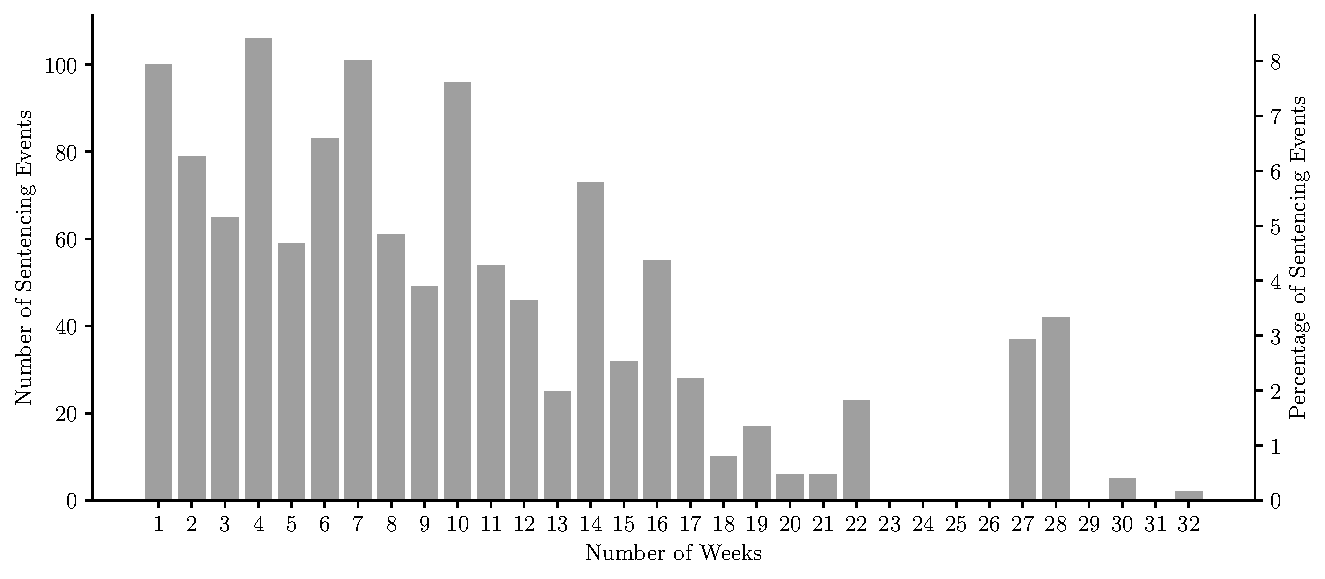
\includegraphics[scale=0.75]{Figures/Missing_Date_Histogram_of_Potential_Week_Histogram}
        \caption{A histogram of the number of weeks the judge visited the county in which the sentencing events missing the \emph{date} data field occurred.}
        \label{Figure_Missing_Date_Histogram_of_Potential_Week_Histogram}
      \end{figure}

  \subsection{Summary Statistics}
Master
\section{Calendar Data}
  \subsection{Data Cleaning}
    We do two things to clean the calendar data:

    \begin{enumerate}
      \item We discard all judge names in the master calendar that are not mapped to a judge number in the sentencing dataset. We discard these judge names because we do not observe any sentencing events for them. The discarded judge names are as follows: Bergdorf, Couch, Drew, Gier, Peeples, Simmons, Watts, and Young. Since we are using the same sentencing data as \cite{hester2017conditional}, we can conclude that they also excluded these judges.
    	\item We combine the schedules of Judges "Cooper" and "Cooper, TW" in the calendar data. There are three judges in the calendar data with last name Cooper: (i) Cooper, (ii) Cooper, TW, and (iii) Cooper, GT. If we run the algorithm proposed in Section \ref{Sec:Mapping_Judge_Numbers_To_Judge_Names} using the master calendar with three distinct judges with last name Cooper, Judge 14 is mapped to either Judge Cooper (under the perfect match criterion) or Judge Cooper, TW (under the overlapping match criterion). Table \ref{Table_Coopers_Schedules} depicts the schedules of the three judges with last name Cooper (according to the master calendar) as well as the counties visited by Judge 14 (according to the sentencing dataset). The counties to which either Judge Cooper or Judge Cooper, TW are assigned are depicted in blue. The counties to which Judge Cooper, GT is assigned are depicted in green. The counties to which neither Judge Cooper, nor Judge Cooper, TW or Cooper, GT are assigned are depicted in red. Table \ref{Table_Coopers_Schedules} shows that the schedules of Judges Cooper and Cooper, TW do not overlap. Moreover, their combined schedules resemble the schedule of Judge 14 (the list of counties visited by Judge 14) the most. This suggests that Judge Cooper and Judge Cooper, TW are (most likely) the same person. Therefore, we combine the schedules of Judges "Cooper" and "Cooper, TW".\footnote{Incidentally, only two judges with last name Cooper are listed on the South Carolina Judicial branch's website. These judges are Thomas W. Cooper, Jr. and G. Thomas Cooper, Jr.; please see \url{https://www.sccourts.org/circuitCourt/displaycirjudge.cfm?judgeid=2054} and \url{https://www.sccourts.org/circuitCourt/displaycirjudge.cfm?judgeid=2126} (accessed on December 14th, 2020) for their bios.}
    \end{enumerate}

    \begin{table}[H]
    	\centering
    	\vspace{-11mm}
    	\hspace*{-16mm}
    	\setlength\tabcolsep{0pt} % default value: 6pt
    	{\footnotesize
    		\begin{tabular}{L{23mm}C{55mm}C{38mm}C{38mm}C{38mm}}
    			\hline
    			\rule{0pt}{2.3ex} Week & Judge 14 & Cooper & Cooper, TW & Cooper, GT \\
    			\hline
    			%\rowgroup{Consumer Surplus} \\
    			%\rule{0pt}{2.3ex} July 3 & & & &\\
    			\rule{0pt}{2.3ex} July 10 & & \textcolor{black}{Aiken} & &\\
    			\rule{0pt}{2.3ex} July 17 & & & &  \textcolor{black}{Berkeley}\\\rule{0pt}{2.3ex} July 24 & & & &  \textcolor{black}{Richland}\\
    			\rule{0pt}{2.3ex} July 31 & & \textcolor{black}{Sumter} & &  \textcolor{black}{Greenville}\\\rule{0pt}{2.3ex} August 7 &  \textcolor{green}{Sumter} & \textcolor{green}{Sumter} & &  \textcolor{black}{Greenwood}\\
    			\rule{0pt}{2.3ex} August 21 &  \textcolor{blue}{Greenville} & \textcolor{black}{Sumter} & &  \textcolor{blue}{Greenville}\\
    			\rule{0pt}{2.3ex} August 28 &  \textcolor{green}{Williamsburg}, \textcolor{red}{Sumter} & \textcolor{green}{Williamsburg}, \textcolor{black}{Orangeburg} & &  \textcolor{black}{Richland}, \textcolor{black}{Greenville}\\
    			\rule{0pt}{2.3ex} September 4 &  \textcolor{green}{Williamsburg}, \textcolor{blue}{Greenville} & \textcolor{green}{Williamsburg} & &  \textcolor{blue}{Greenville}\\
    			\rule{0pt}{2.3ex} September 11 &  \textcolor{green}{Sumter}, \textcolor{red}{Clarendon}, \textcolor{blue}{Greenville} & \textcolor{green}{Sumter} & &  \textcolor{blue}{Greenville}\\
    			\rule{0pt}{2.3ex} September 18 & & & &  \textcolor{black}{Spartanburg}\\
    			\rule{0pt}{2.3ex} September 25 &  \textcolor{blue}{Greenville} & \textcolor{black}{Williamsburg} & &  \textcolor{blue}{Greenville}\\
    			\rule{0pt}{2.3ex} October 9 &  \textcolor{green}{Lee}, \textcolor{red}{Sumter} & \textcolor{green}{Lee} & &  \textcolor{black}{Richland}\\
    			\rule{0pt}{2.3ex} October 16 &  \textcolor{green}{Williamsburg} & \textcolor{green}{Williamsburg}, \textcolor{black}{Aiken} & &  \textcolor{black}{Richland}\\
    			\rule{0pt}{2.3ex} October 23 &  \textcolor{green}{Williamsburg}, \textcolor{red}{Horry}, \textcolor{red}{Georgetown} & \textcolor{green}{Williamsburg} & &\\
    			\rule{0pt}{2.3ex} October 30 &  \textcolor{green}{Sumter} & \textcolor{green}{Sumter} & &  \textcolor{black}{Richland}\\
    			\rule{0pt}{2.3ex} November 6 & & \textcolor{black}{Williamsburg} & &  \textcolor{black}{Richland}\\\rule{0pt}{2.3ex} November 13 &  \textcolor{green}{Sumter} & \textcolor{green}{Sumter} & &\\
    			\rule{0pt}{2.3ex} November 27 & & \textcolor{black}{Clarendon} & &  \textcolor{black}{Newberry}\\
    			\rule{0pt}{2.3ex} December 4 &  \textcolor{green}{Lee}, \textcolor{red}{Sumter} & \textcolor{green}{Lee} & &\\
    			\rule{0pt}{2.3ex} December 11 &  \textcolor{green}{Lee} & \textcolor{green}{Lee}, \textcolor{black}{Aiken} & &\\
    			\rule{0pt}{2.3ex} January 1 & & & \textcolor{black}{Aiken} &\\
    			\rule{0pt}{2.3ex} January 8 &  \textcolor{green}{Richland} & & \textcolor{green}{Richland}, \textcolor{black}{Aiken} &  \textcolor{black}{McCormick}\\
    			\rule{0pt}{2.3ex} January 15 & & & \textcolor{black}{Kershaw} &\\
    			\rule{0pt}{2.3ex} January 22 & & & \textcolor{black}{Aiken} &\\
    			\rule{0pt}{2.3ex} January 29 &  \textcolor{green}{Aiken} & & \textcolor{black}{Beaufort}, \textcolor{green}{Aiken} &  \textcolor{black}{Lexington}\\
    			\rule{0pt}{2.3ex} February 5 & & & \textcolor{black}{Orangeburg} &  \textcolor{black}{Laurens}\\
    			\rule{0pt}{2.3ex} February 12 & & & &  \textcolor{black}{Newberry}\\
    			\rule{0pt}{2.3ex} February 26 &  \textcolor{green}{Richland} & & \textcolor{green}{Richland}, \textcolor{black}{Orangeburg} &  \textcolor{black}{Greenville}\\
    			\rule{0pt}{2.3ex} March 5 &  \textcolor{red}{Richland}, \textcolor{blue}{Edgefield} & & &  \textcolor{black}{McCormick}, \textcolor{blue}{Edgefield}\\
    			\rule{0pt}{2.3ex} March 12 & & & \textcolor{black}{Orangeburg} &\\
    			\rule{0pt}{2.3ex} March 19 &  \textcolor{green}{Orangeburg} & & \textcolor{green}{Orangeburg} &\\
    			\rule{0pt}{2.3ex} March 26 &  \textcolor{green}{Richland} & & \textcolor{green}{Richland} &  \textcolor{black}{Edgefield}\\
    			\rule{0pt}{2.3ex} April 9 &  \textcolor{green}{Richland} & & \textcolor{green}{Richland} &  \textcolor{black}{Lexington}\\
    			\rule{0pt}{2.3ex} April 16 &  \textcolor{red}{Richland} & & &\\
    			\rule{0pt}{2.3ex} April 23 & & & \textcolor{black}{Richland} &  \textcolor{black}{Lexington}\\
    			\rule{0pt}{2.3ex} April 30 &  \textcolor{green}{Kershaw} & & \textcolor{green}{Kershaw} &  \textcolor{black}{Lexington}\\
    			\rule{0pt}{2.3ex} May 14 & & & &  \textcolor{black}{Lexington}\\\rule{0pt}{2.3ex} May 21 &  \textcolor{green}{Richland} & & \textcolor{green}{Richland} &  \textcolor{black}{Edgefield}\\
    			\rule{0pt}{2.3ex} May 28 &  \textcolor{green}{Richland} & & \textcolor{green}{Richland} &\\
    			\rule{0pt}{2.3ex} June 4 &  \textcolor{green}{Richland} & & \textcolor{green}{Richland} &  \textcolor{black}{Edgefield}\\
    			\rule{0pt}{2.3ex} June 11 & & & &  \textcolor{black}{Edgefield}\\\rule{0pt}{2.3ex} June 18 &  \textcolor{green}{Kershaw} & & \textcolor{green}{Kershaw} &  \textcolor{black}{Lexington}\\
    			\rule{0pt}{2.3ex} June 25 & & & \textcolor{black}{Richland} &  \textcolor{black}{McCormick}\\
    			\hline
    		\end{tabular}
    	}
    	\vspace{-1mm}
    	\caption{The list of counties visited by Judge 14 (according to the sentencing dataset) and the counties visited by Judges Cooper, Cooper, TW, and Cooper, GT (according to the master calendar). The counties visited by Judge 14 to which either Judge Cooper or Judge Cooper, TW were assigned are written in green font. The counties visited by Judge 14 to which Judge Cooper, GT was assigned are written in blue font. The counties visited by Judge 14 to which neither Judge Cooper, nor Judge Cooper, TW or Cooper, GT were assigned are written in red font. For visual clarity, only the weeks in which at least one judge has an assignment or sentencing event are depicted.}
    	\label{Table_Coopers_Schedules}
    	\vspace{-2mm}
    \end{table}

\section{Discrepancies between the Sentencing Data and the Master Calendar Data}
  \label{Sec:Master_Calendar:Further_Analysis_of_Some_Assignments}

  This section studies the discrepancies between the sentencing data and the calendar data. In doing so, we take advantage of the mapping from judge numbers to judge names (discussed in Section \ref{mapping-judge-names}).

  \subsection{No Assignments Case}
    \label{Sec:Master_Calendar:Further_Analysis_of_Some_Assignments:Category_i}
    There are 110 judge-week combinations in this category. We observe no sentencing events (in the sentencing dataset) for 101 out of these 110 ($91.8\%$) judge-week combinations. Recall that the judges in these combinations have no assignments on the master calendar. Therefore, there are no inconsistencies between the master calendar and the sentencing dataset for these 101 judge-week combinations. The remaining 9 judge-week combinations are listed in Table \ref{Table_Mater_Calendar_Problematic_Cases_Detailed_Category_i}. We observe at least one sentencing event (in the sentencing dataset) for these judge-week combinations. Each judge visits only one county (according to the sentencing dataset) in these 9 judge-week combinations.

    \begin{table}[H]
      \centering
      \caption{Judge-week combinations in which the judge has sentencing events in a county to which he is not assigned - "No Assignment" category. The first number in the parenthesis depicts the number of pleas and the second number depicts the number of trials.}
      \vspace{-2mm}
      \hspace*{0mm}
      \setlength\tabcolsep{0pt} % default value: 6pt
      {\scriptsize
        \begin{tabular}{>{\quad}L{6mm}C{8mm}C{2mm}L{17mm}C{25mm}C{25mm}C{25mm}C{25mm}C{25mm}cccc}
          \toprule
          & & && \multicolumn{5}{c}{Sentencing Data Set} \\
          \cmidrule(ll){5-9}
          & Judge && Week & Monday & Tuesday & Wednesday & Thursday & Friday \\
          \midrule
          1 &   7 & {} &  2000-07-03 &                                    &                                    &                                    &                                    &  \textcolor{red}{Dorchester (0,1)} \\
2 &   7 & {} &  2000-07-24 &  \textcolor{red}{Orangeburg (1,0)} &  \textcolor{red}{Orangeburg (1,0)} &                                    &  \textcolor{red}{Orangeburg (1,0)} &                                    \\
3 &   7 & {} &  2001-01-29 &  \textcolor{red}{Dorchester (1,0)} &                                    &                                    &                                    &                                    \\
4 &   7 & {} &  2001-06-04 &  \textcolor{red}{Orangeburg (5,0)} &                                    &  \textcolor{red}{Orangeburg (2,1)} &  \textcolor{red}{Orangeburg (4,0)} &                                    \\
5 &  25 & {} &  2000-10-30 &                                    &                                    &   \textcolor{red}{Greenwood (1,0)} &                                    &                                    \\
6 &  25 & {} &  2001-04-23 &   \textcolor{red}{Greenwood (1,0)} &                                    &                                    &                                    &                                    \\
7 &  42 & {} &  2001-03-12 &                                    &                                    &  \textcolor{red}{Greenville (1,0)} &                                    &                                    \\
8 &  42 & {} &  2001-04-16 &                                    &  \textcolor{red}{Greenville (1,0)} &                                    &                                    &                                    \\
9 &  46 & {} &  2000-10-23 &  \textcolor{red}{Charleston (1,0)} &                                    &                                    &                                    &                                    \\

          \bottomrule
        \end{tabular}
      }
      \label{Table_Mater_Calendar_Problematic_Cases_Detailed_Category_i}
    \end{table}

  \subsection{Single Assignment Case}
    \label{Sec:Master_Calendar:Further_Analysis_of_Some_Assignments:Category_ii}
    \subsubsection{Single assignment, no dates}
      We start with the single assignment, no date category. There are 2,214 judge-week combinations in this category. Although in single assignment, no date judge-week combinations (according to the master calendar) the judges have an assignment the entire week, they do not necessarily sentence every day of the week. For 1871 of the 2200 ($85\%$) judge-week combinations, we only observe sentencing events in the county to which the judge is assigned, i.e., we do not observe sentencing events in a county other than the county to which the judge is assigned. In other words, there are no inconsistencies between the master calendar and the sentencing dataset for 1871 of these 2200 judge-week combinations. The remaining 328 judge-week combinations are listed in Table \ref{Table_Mater_Calendar_Problematic_Cases_Detailed_Category_i}. We observe at least one sentencing event (in the sentencing dataset) in a county to which the judge is not assigned in these judge-week combinations.

      \begin{table}[H]
        \centering
        \caption{Judge-week combinations in which the judge has sentencing events in a county to which he is not assigned - single assignment, no date category. The counties written in green font are the counties to which the judge is assigned. The counties written in red font are the counties to which the judge is not assigned. The counties written in blue font are the counties to which the judge is not assigned, however, he is assigned to the circuit court containing these counties. So, the county assignment in the master calendar and this county belong to the same circuit court.}
        \vspace{-2mm}
        \hspace*{-26.5mm}
        \setlength\tabcolsep{2pt} % default value: 6pt
        {\scriptsize
          \begin{tabular}{>{\quad}C{8mm}C{8mm}L{20mm}L{31mm}C{24mm}C{22mm}C{24mm}C{25mm}C{23mm}}
            \toprule
            & & & & \multicolumn{5}{c}{Sentencing Data Set} \\
            \cmidrule(ll){5-9}
            & Judge & Week & Master Calendar & Monday & Tuesday & Wednesday & Thursday & Friday \\
            \midrule
            1   &   1 &  2000-08-07 &            York GS &                                                                        &                                        \textcolor{green}{York (2,0)} &                                    \textcolor{green}{York (2,0)} &                                           \textcolor{green}{York (4,0)} &       \textcolor{red}{Kershaw (1,0)}, \textcolor{green}{York (7,0)} \\
2   &   1 &  2000-08-21 &            York GS &                                                                        &                                        \textcolor{green}{York (1,0)} &                                                                  &                                                                         &        \textcolor{blue}{Union (1,0)}, \textcolor{green}{York (2,0)} \\
3   &   1 &  2000-09-11 &            York GS &                                          \textcolor{green}{York (6,0)} &                                        \textcolor{green}{York (2,0)} &                                                                  &                                           \textcolor{green}{York (2,0)} &   \textcolor{red}{Spartanburg (1,0)}, \textcolor{green}{York (5,0)} \\
4   &   1 &  2000-10-09 &            York GS &                                                                        &                                                                      &  \textcolor{red}{Fairfield (1,0)}, \textcolor{green}{York (1,0)} &                                           \textcolor{green}{York (5,0)} &                                       \textcolor{green}{York (4,0)} \\
5   &   1 &  2000-10-23 &            York GS &                                          \textcolor{green}{York (2,0)} &                                        \textcolor{green}{York (3,0)} &                                    \textcolor{green}{York (9,0)} &                                           \textcolor{green}{York (1,0)} &       \textcolor{red}{Kershaw (1,0)}, \textcolor{green}{York (6,0)} \\
6   &   1 &  2001-01-08 &         Chester GS &                                       \textcolor{green}{Chester (2,0)} &                                          \textcolor{red}{York (1,0)} &                                                                  &                                                                         &                                    \textcolor{green}{Chester (2,0)} \\
7   &   1 &  2001-02-12 &         Chester CP &                                                                        &                                                                      &                                                                  &                                       \textcolor{blue}{Lancaster (1,0)} &                                                                     \\
8   &   1 &  2001-06-04 &         Chester GS &                                                                        &                                                                      &                                 \textcolor{green}{Chester (0,1)} &    \textcolor{green}{Chester (2,0)}, \textcolor{red}{Spartanburg (1,0)} &                                    \textcolor{green}{Chester (3,0)} \\
9   &   2 &  2000-07-24 &        Richland GS &                                      \textcolor{green}{Richland (4,0)} &  \textcolor{red}{Lexington (1,0)}, \textcolor{green}{Richland (4,0)} &                                \textcolor{green}{Richland (2,0)} &                                       \textcolor{green}{Richland (7,0)} &                                                                     \\
10  &   2 &  2000-09-11 &        Richland GS &                                                                        &   \textcolor{blue}{Kershaw (1,0)}, \textcolor{green}{Richland (6,0)} &                                \textcolor{green}{Richland (7,0)} &                                       \textcolor{green}{Richland (3,0)} &                                   \textcolor{green}{Richland (1,0)} \\
.   &   . &           . &                  . &                                                                      . &                                                                    . &                                                                . &                                                                       . &                                                                   . \\
320 &  49 &  2001-06-25 &        Richland GS &    \textcolor{red}{Lexington (1,0)}, \textcolor{green}{Richland (1,0)} &                                                                      &                                                                  &                                                                         &                                                                     \\
321 &  50 &  2000-09-25 &        Richland GS &                                      \textcolor{green}{Richland (7,0)} &   \textcolor{red}{Clarendon (1,0)}, \textcolor{red}{Lexington (1,0)} &                                \textcolor{green}{Richland (2,1)} &                                       \textcolor{green}{Richland (3,0)} &                                   \textcolor{green}{Richland (1,0)} \\
322 &  50 &  2000-10-02 &        in chambers &                                                                        &                                                                      &                                                                  &                                                                         &                                     \textcolor{red}{Richland (1,0)} \\
323 &  50 &  2000-10-16 &      Orangeburg GS &                                   \textcolor{green}{Orangeburg (14,0)} &                                  \textcolor{green}{Orangeburg (2,0)} &                              \textcolor{green}{Orangeburg (5,0)} &  \textcolor{red}{Charleston (1,0)}, \textcolor{green}{Orangeburg (3,0)} &                                 \textcolor{green}{Orangeburg (1,0)} \\
324 &  50 &  2000-12-18 &        in chambers &                                        \textcolor{red}{Richland (1,0)} &                                     \textcolor{red}{Richland (24,0)} &                                                                  &                                                                         &                                                                     \\
325 &  50 &  2001-01-08 &      Orangeburg GS &  \textcolor{blue}{Calhoun (2,0)}, \textcolor{green}{Orangeburg (14,0)} &                                  \textcolor{green}{Orangeburg (3,0)} &                              \textcolor{green}{Orangeburg (4,0)} &                                     \textcolor{green}{Orangeburg (3,0)} &   \textcolor{red}{Aiken (1,0)}, \textcolor{green}{Orangeburg (2,0)} \\
326 &  50 &  2001-01-22 &          Sumter GS &           \textcolor{green}{Sumter (6,0)}, \textcolor{red}{York (1,0)} &                                      \textcolor{green}{Sumter (2,0)} &                                  \textcolor{green}{Sumter (3,0)} &                                         \textcolor{green}{Sumter (1,0)} &                                     \textcolor{green}{Sumter (3,0)} \\
327 &  50 &  2001-02-05 &       Clarendon GS &                                     \textcolor{green}{Clarendon (3,0)} &                                   \textcolor{green}{Clarendon (2,0)} &                               \textcolor{green}{Clarendon (1,0)} &                                                                         &  \textcolor{green}{Clarendon (3,0)}, \textcolor{blue}{Sumter (1,0)} \\
328 &  50 &  2001-04-16 &          Sumter GS &     \textcolor{blue}{Clarendon (0,1)}, \textcolor{green}{Sumter (5,0)} &                                      \textcolor{green}{Sumter (3,0)} &                                  \textcolor{green}{Sumter (2,0)} &                                         \textcolor{green}{Sumter (3,0)} &                                     \textcolor{green}{Sumter (3,0)} \\
329 &  50 &  2001-05-28 &  3rd Cir. CPNJ/PCR &                                                                        &                                                                      &                                                                  &                                          \textcolor{blue}{Sumter (1,0)} &                                \textcolor{blue}{Williamsburg (1,0)} \\

            \bottomrule
          \end{tabular}
        }
        \label{Table_Mater_Calendar_Problematic_Cases_Detailed_Category_iia}
      \end{table}

    \subsubsection{Single assignment with dates}
      There are 14 judge-week combinations in Category ii (b), i.e., a single assignment with specific dates. In 10 of the 14 judge-week combinations, we either observe no sentencing events or sentencing events only in the same county as listed in the master calendar (2 of them). In other words, there are no inconsistencies between the master calendar and the sentencing dataset for 10 of these 14 ($71.4\%$) judge-week combinations. The remaining 4 judge-week combinations are listed in Table \ref{Table_Mater_Calendar_Problematic_Cases_Detailed_Category_i}. In these 4 judge-week combinations, exactly one of the following conditions holds:
      \begin{enumerate}
        \item At least one sentencing event occurred in a county not stated on the master calendar (3 judge-week combinations); see the last three rows of Table \ref{Table_Mater_Calendar_Problematic_Cases_Detailed_Category_iib}.
        \item At least one sentencing event occurred in the county stated on the master calendar but on a date not stated on the master calendar (1 judge-week combination); see the first row of Table \ref{Table_Mater_Calendar_Problematic_Cases_Detailed_Category_iib}.
      \end{enumerate}

      \begin{table}[H]
        \centering
        \caption{Judge-week combinations in which the judge has sentencing events in a county to which he is not assigned - single assignment, with dates category. The counties written in green font are the counties to which the judge is assigned. The counties written in red font are the counties to which the judge is not assigned.}
        \vspace{-2mm}
        \hspace*{-21mm}
        \setlength\tabcolsep{2pt} % default value: 6pt
        {\scriptsize
          \begin{tabular}{>{\quad}C{6mm}C{8mm}L{18mm}L{31mm}C{22mm}C{22mm}C{22mm}C{22mm}C{22mm}}
            \toprule
            & & & & \multicolumn{5}{c}{Sentencing Data Set}\\
            \cmidrule(ll){5-9}
            & Judge & Week & Master Calendar & Monday & Tuesday & Wednesday & Thursday & Friday\\
            \midrule
            1 &   6 &  2001-03-19 &     Horry GS CP CC 21,22,23 &                                                                &      \textcolor{red}{Horry (6,0)} &                                    &                                       \textcolor{green}{Horry (5,0)} &                                   \\
2 &  27 &  2000-09-25 &   Bamberg GS 25,26,27,28,29 &  \textcolor{green}{Bamberg (10,0)}, \textcolor{red}{Lee (1,0)} &  \textcolor{green}{Bamberg (6,0)} &                                    &                                                                      &                                   \\
3 &  46 &  2000-10-30 &           Barnwell GS 1,2,3 &                                                                &                                   &  \textcolor{green}{Barnwell (1,0)} &  \textcolor{red}{Allendale (1,0)}, \textcolor{green}{Barnwell (2,0)} &                                   \\
4 &  48 &  2000-10-23 &  13th Cir. CPNJ 23,24,25,26 &                                                                &                                   &                                    &                                                                      &  \textcolor{red}{Clarendon (1,0)} \\

            \bottomrule
          \end{tabular}
        }
        \label{Table_Mater_Calendar_Problematic_Cases_Detailed_Category_iib}
      \end{table}

  \subsection{Multiple Assignments Case}
    \label{Sec:Master_Calendar:Further_Analysis_of_Some_Assignments:Category_iii}
    \subsubsection{Multiple assignments, no dates}
      We start with the category multiple assignment, no dates. There are 19 judge-week combinations in this category. For 17 of the 19 ($89.4\%$) judge-week combinations in this category, we only observe sentencing events in one of the two counties stated on the master calendar. In other words, there are no inconsistencies between the master calendar and the sentencing dataset for 17 of these 19 judge-week combinations. The remaining 2 judge-week combinations are listed in Table \ref{Table_Mater_Calendar_Problematic_Cases_Detailed_Category_iii_a}. The judge-week combinations in this category that satisfy (at least) one of the following conditions are potentially problematic:
      \begin{enumerate}
        \item At least one sentencing event occurred in a county not stated on the master calendar (Both rows of Table \ref{Table_Mater_Calendar_Problematic_Cases_Detailed_Category_iii_a}).
        \item The judge sentenced in more than one county on a day (First row of Table \ref{Table_Mater_Calendar_Problematic_Cases_Detailed_Category_iii_a}).
      \end{enumerate}

      \begin{table}[H]
        \centering
        \caption{Judge-week combinations in which the judge has sentencing events in a county to which he is not assigned - multiple assignment, no dates cateogry. The county written in green font is the county to which the judge is assigned. The counties written in blue font are the counties to which the judge is not assigned, however, he is assigned to the circuit court containing this county. So, the county assignment in the master calendar and this county belong to the same circuit court.}
        \vspace{-2mm}
        \hspace*{-0mm}
        \setlength\tabcolsep{2pt} % default value: 6pt
        {\scriptsize
          \begin{tabular}{>{\quad}C{6mm}C{8mm}L{16mm}L{25mm}C{15mm}C{15mm}C{20mm}C{17mm}C{17mm}}
            \toprule
            & & & & \multicolumn{5}{c}{Sentencing Data Set} \\
            \cmidrule(ll){5-9}
            & Judge & Week & Master Calendar & Monday & Tuesday & Wednesday & Thursday & Friday \\
            \midrule
            1 &  2 &  2001-04-30 &  Aiken GS CC, 2nd Cir. CP/PCR &   &   &  \textcolor{green}{Aiken (5,0)}, \textcolor{blue}{Bamberg (1,0)} &                                 &   \\
2 &  9 &  2001-01-08 &           Florence GS, Lee GS &   &   &                                   \textcolor{blue}{Marion (1,0)} &  \textcolor{blue}{Marion (1,0)} &   \\

            \bottomrule
          \end{tabular}
        }
        \label{Table_Mater_Calendar_Problematic_Cases_Detailed_Category_iii_a}
      \end{table}

    \subsubsection{Multiple assignments, some dates}
      There are 181 judge-week combinations in the multiple assignment, some dates category. For 155 of these 181 ($85.6\%$) judge-week combinations, we only observe sentencing events in one of the two counties stated on the master calendar and only on the days stated on the master calendar. In other words, there are no inconsistencies between the master calendar and the sentencing dataset for 155 of these 181 judge-week combinations. The remaining 26 judge-week combinations are listed in Table \ref{Table_Mater_Calendar_Problematic_Cases_Detailed_Category_iii_b}. There is only one judge-week combination in the multiple assignment, some dates ambiguous category, and we do not observe any conflicts in that week.

      \begin{table}[H]
        \centering
        \caption{Judge-week combinations in which the judge has sentencing events in a county to which he is not assigned - multiple assignment, some dates category. The counties written in green font are the counties to which the judge is assigned. The counties written in red font are the counties to which the judge is not assigned. The counties written in blue font are the counties to which the judge is not assigned, however, he is assigned to the circuit court containing these counties. So, the county assignment in the master calendar and this county belong to the same circuit court.}
        \vspace{-2mm}
        \hspace*{-21mm}
        \setlength\tabcolsep{2pt} % default value: 6pt
        {\scriptsize
          \begin{tabular}{>{\quad}C{6mm}C{8mm}L{17mm}L{30mm}C{22mm}C{22mm}C{24mm}C{23mm}C{22mm}}
            \toprule
            & & & & \multicolumn{5}{c}{Sentencing Data Set} \\
            \cmidrule(ll){5-9}
            & Judge & Week & Master Calendar & Monday & Tuesday & Wednesday & Thursday & Friday \\
            \midrule
            1  &   6 &  2000-10-16 &                       Florence CP, Florence GS CC 20 &                                                                       &                                                                                                       &                                                                            &                                        \textcolor{red}{Horry (1,0)} &                                      \textcolor{green}{Florence (8,0)} \\
2  &   6 &  2000-12-18 &                    in chambers, 12th Cir. CPNJ 18,19 &                                        \textcolor{blue}{Marion (1,0)} &                                                                                                       &                                                                            &                                                                     &                                                                        \\
3  &   9 &  2001-06-18 &                          Florence GS, Florence CP 21 &                                     \textcolor{green}{Florence (5,0)} &                                                                     \textcolor{green}{Florence (3,0)} &      \textcolor{red}{Darlington (1,0)}, \textcolor{green}{Florence (17,0)} &                                  \textcolor{green}{Florence (12,0)} &                                      \textcolor{green}{Florence (5,0)} \\
4  &  10 &  2000-10-02 &                     in chambers, 7th Cir. CPNJ 2,3,5 &                                                                       &                                                                                                       &                                                                            &                                 \textcolor{blue}{Spartanburg (3,0)} &                                                                        \\
5  &  10 &  2001-06-04 &                   8th Cir. CPNJ, Spartanburg GS CC 8 &                                       \textcolor{blue}{Laurens (1,0)} &                                                                                                       &                                                                            &                                                                     &                                                                        \\
6  &  12 &  2001-03-05 &                      McCormick GS, Edgefield GS CC 8 &                                    \textcolor{green}{McCormick (3,0)} &                                                                                                       &                                                                            &                                      \textcolor{blue}{Saluda (1,0)} &                                                                        \\
7  &  13 &  2000-08-28 &                  Williamsburg GS, Orangeburg GS CC 1 &                                 \textcolor{green}{Williamsburg (3,0)} &                                                                 \textcolor{green}{Williamsburg (4,0)} &      \textcolor{blue}{Sumter (1,0)}, \textcolor{green}{Williamsburg (2,0)} &                               \textcolor{green}{Williamsburg (6,0)} &                                                                        \\
8  &  13 &  2000-12-11 &                               Lee GS, Aiken GS CC 15 &                                          \textcolor{green}{Lee (1,0)} &                                                                          \textcolor{green}{Lee (1,0)} &                                                                            &                                                                     &                                             \textcolor{red}{Lee (0,2)} \\
9  &  13 &  2001-01-08 &                          Richland GS, Aiken GS CC 12 &                                     \textcolor{green}{Richland (8,0)} &                                                                     \textcolor{green}{Richland (3,0)} &                                          \textcolor{green}{Richland (1,0)} &                                                                     &                                        \textcolor{red}{Richland (0,1)} \\
10 &  17 &  2001-03-12 &                    Spartanburg CP, Cherokee GS CC 15 &                                                                       &                                                                                                       &                                             \textcolor{red}{Pickens (1,0)} &                                   \textcolor{green}{Cherokee (1,0)} &                                                                        \\
11 &  25 &  2001-02-26 &                    Greenwood GS, 8th Cir. CPNJ CC 26 &                                     \textcolor{blue}{Greenwood (4,0)} &                                                                   \textcolor{green}{Greenwood (10,0)} &                                         \textcolor{green}{Greenwood (7,0)} &  \textcolor{blue}{Abbeville (1,0)}, \textcolor{blue}{Laurens (1,0)} &  \textcolor{red}{Greenville (1,0)}, \textcolor{green}{Greenwood (5,0)} \\
12 &  26 &  2000-11-13 &                             Greenwood GS, Medical 17 &                                       \textcolor{red}{Anderson (1,0)} &                                                                                                       &                                         \textcolor{green}{Greenwood (9,1)} &                                  \textcolor{green}{Greenwood (5,0)} &                                                                        \\
13 &  28 &  2000-07-31 &                       Richland GS, Lexington GS CC 3 &  \textcolor{red}{Lexington (1,0)}, \textcolor{green}{Richland (13,0)} &  \textcolor{blue}{Kershaw (1,0)}, \textcolor{red}{Marlboro (1,0)}, \textcolor{green}{Richland (10,0)} &                                         \textcolor{green}{Richland (12,0)} &                                     \textcolor{red}{Richland (4,0)} &                                                                        \\
14 &  28 &  2001-03-19 &                       Darlington GS, Dillon GS CC 23 &                                   \textcolor{green}{Darlington (1,0)} &                                                                   \textcolor{green}{Darlington (8,0)} &  \textcolor{blue}{Chesterfield (1,0)}, \textcolor{green}{Darlington (9,0)} &                                 \textcolor{green}{Darlington (3,0)} &                                                                        \\
15 &  29 &  2001-06-04 &                    16th Cir. CPNJ, Clarendon GS CC 8 &                                                                       &                                                                         \textcolor{blue}{Union (1,0)} &                                                                            &                                                                     &                                     \textcolor{green}{Clarendon (1,0)} \\
16 &  30 &  2000-10-02 &                         in chambers, Greenville GS 6 &                                                                       &                                                                                                       &                                            \textcolor{red}{Anderson (1,0)} &                                                                     &                                                                        \\
17 &  32 &  2001-04-09 &                        Charleston CP, Horry GS CC 9  &                                     \textcolor{red}{Charleston (1,0)} &                                                                                                       &                                                                            &                                                                     &                                                                        \\
18 &  32 &  2001-04-30 &                        Berkeley GS, Richland GS CC 2 &                                     \textcolor{green}{Berkeley (6,0)} &                                                                     \textcolor{green}{Berkeley (1,0)} &                                            \textcolor{red}{Berkeley (2,0)} &                                   \textcolor{green}{Berkeley (6,0)} &                                                                        \\
19 &  34 &  2001-04-16 &                     Florence GS, 5th Cir. CPNJ CC 20 &                                    \textcolor{green}{Florence (12,0)} &                                                                     \textcolor{green}{Florence (8,0)} &                                         \textcolor{green}{Florence (16,0)} &                                   \textcolor{green}{Florence (5,0)} &                                        \textcolor{red}{Florence (5,0)} \\
20 &  34 &  2001-05-14 &                       Marion GS, 5th Cir. CPNJ CC 14 &                                         \textcolor{red}{Marion (7,0)} &                                                                                                       &                                            \textcolor{green}{Marion (1,0)} &                                                                     &                                        \textcolor{green}{Marion (8,0)} \\
21 &  37 &  2001-01-15 &                   Georgetown CP, Georgetown GS CC 19 &                                                                       &                                                                                                       &                                                                            &                                       \textcolor{red}{Marion (0,2)} &                                                                        \\
22 &  39 &  2000-08-28 &                          Anderson CP, Oconee GS CC 1 &                                                                       &                                                                                                       &                                                                            &                                                                     &                                       \textcolor{blue}{Anderson (1,0)} \\
23 &  39 &  2000-11-06 &                     Anderson GS, 10th Cir. CPNJ CC 8 &  \textcolor{green}{Anderson (3,0)}, \textcolor{red}{Greenville (1,0)} &                                                                                                       &                                           \textcolor{blue}{Anderson (8,0)} &                                  \textcolor{green}{Anderson (10,0)} &                                                                        \\
24 &  40 &  2001-05-07 &  in chambers, Greenville GS(SGJ) 7, 13th Cir. CPNJ 8 &                                    \textcolor{red}{Spartanburg (1,0)} &                                                                                                       &                                                                            &                                                                     &                                                                        \\
25 &  43 &  2001-05-07 &                         in chambers, 9th Cir. CPNJ 8 &                                                                       &                                                                       \textcolor{red}{Colleton (0,1)} &                                                                            &                                                                     &                                                                        \\
26 &  47 &  2000-12-04 &                     15th Cir. CPNJ, Horry GS CP CC 5 &                                         \textcolor{blue}{Horry (1,0)} &                                                                                                       &                                                                            &                                                                     &                                                                        \\

            \bottomrule
          \end{tabular}
        }
        \label{Table_Mater_Calendar_Problematic_Cases_Detailed_Category_iii_b}
      \end{table}

      The judge-week combinations listed in Table \ref{Table_Mater_Calendar_Problematic_Cases_Detailed_Category_iii_b} satisfy (at least) one of the following conditions, which are problematic (some satisfy multiple conditions):\footnote{For example, judge-week combination 12 satisfies all four conditions. In judge-week combination 12, the assignment of Judge 29 in the week of July 31 is Richland GS and Lexington GS CC 3. Therefore, we would expect Judge 29 to be in Lexington on Thursday, and to be in Richland on Monday, Tuesday, Wednesday, and Friday. Since we observe sentencing events in Marlboro and Kershaw (alongside Richland) on Tuesday, judge-week combination 12 satisfies Conditions 1 and 4. Since we observe sentencing events in both Lexington and Richland on Monday, judge-week combination 12 satisfies Condition 3. Since we observe sentencing events in Richland on Thursday, judge-week combination 12 satisfies Condition 2, as well.}

        \begin{enumerate}
          \item At least one sentencing event occurred in a county not stated on the master calendar, e.g., judge-week combination 2 of Table \ref{Table_Mater_Calendar_Problematic_Cases_Detailed_Category_iii_b} (17 such judge-week combinations are listed in Table \ref{Table_Mater_Calendar_Problematic_Cases_Detailed_Category_iii_b}).
          \item At least one sentencing event occurred in the county stated on the master calendar with specific dates, but on a date other than the dates specified, e.g., judge-week combination 23 of Table \ref{Table_Mater_Calendar_Problematic_Cases_Detailed_Category_iii_b} (4 such judge-week combinations are listed in Table \ref{Table_Mater_Calendar_Problematic_Cases_Detailed_Category_iii_b}.).
          \item At least one sentencing event occurred in the county stated on the master calendar without specific dates. However, this sentencing event occurred on a date specified for the other county, e.g., judge-week combination 8 of Table \ref{Table_Mater_Calendar_Problematic_Cases_Detailed_Category_iii_b} (8 such judge-week combinations are listed in Table \ref{Table_Mater_Calendar_Problematic_Cases_Detailed_Category_iii_b}.).
          \item The judge sentenced in more than one county on a day, e.g., judge-week combination 3 of Table \ref{Table_Mater_Calendar_Problematic_Cases_Detailed_Category_iii_b} (5 such judge-week combinations are listed in Table \ref{Table_Mater_Calendar_Problematic_Cases_Detailed_Category_iii_b}.).
      \end{enumerate}

    \subsubsection{Multiple assignments, all dates}
      There are 57 judge-week combinations in the multiple assignment, all dates category. For 47 of these 57 ($82.4\%$) judge-week combinations, we only observe sentencing events in one of the two counties stated on the master calendar and only on the days stated on the master calendar. In other words, there are no inconsistencies between the master calendar and the sentencing dataset for 47 of these 57 judge-week combinations. The remaining 10 judge-week combinations are listed in Table \ref{Table_Mater_Calendar_Problematic_Cases_Detailed_Category_iii_c}.

      \begin{table}[H]
        \centering
        \caption{Judge-week combinations in which the judge has sentencing events in a county to which he is not assigned - multiple assignment, all dates category. The counties written in green font are the counties to which the judge is assigned. The counties written in red font are the counties to which the judge is not assigned. The counties written in blue font are the counties to which the judge is not assigned, however, he is assigned to the circuit court containing these counties. So, the county assignment in the master calendar and this county belong to the same circuit court.}
        \vspace{-2mm}
        \hspace*{-20mm}
        \setlength\tabcolsep{2pt} % default value: 6pt
        {\scriptsize
          \begin{tabular}{>{\quad}C{6mm}C{8mm}L{17mm}L{29mm}C{22mm}C{22mm}C{22mm}C{23mm}C{22mm}}
            \toprule
            & & & & \multicolumn{5}{c}{Sentencing Data Set}\\
            \cmidrule(ll){5-9}
            & Judge & Week & Master Calendar & Monday & Tuesday & Wednesday & Thursday & Friday \\
            \midrule
            1  &   5 &  2000-10-16 &                          15th Cir. AW 16,19,20, Aiken 17,18 &                                    &                                                                     \textcolor{green}{Aiken (11,0)} &      \textcolor{green}{Aiken (11,0)} &         \textcolor{blue}{Horry (6,0)}, \textcolor{red}{Williamsburg (1,0)} &       \textcolor{blue}{Horry (1,0)} \\
2  &   9 &  2000-07-10 &                            Darlington GS 11,12,13,14, XX 10 &                                    &                                                                 \textcolor{green}{Darlington (2,0)} &  \textcolor{green}{Darlington (5,0)} &  \textcolor{blue}{Chesterfield (1,0)}, \textcolor{green}{Darlington (9,0)} &                                     \\
3  &  16 &  2000-11-27 &                                  XX 1, Aiken GS 27,28,29,30 &     \textcolor{green}{Aiken (3,0)} &                                                                                                     &       \textcolor{green}{Aiken (1,1)} &         \textcolor{green}{Aiken (7,0)}, \textcolor{red}{Spartanburg (1,0)} &                                     \\
4  &  17 &  2001-04-16 &                 13th Cir. CPNJ 16, Lexington GS 17,18,19,20 &                                    &                                                                                                     &  \textcolor{green}{Lexington (12,0)} &       \textcolor{green}{Lexington (11,0)}, \textcolor{red}{Richland (1,0)} &                                     \\
5  &  26 &  2001-05-28 &              10th Cir. CPNJ/PCR 28,29,30, Lexington GS 31,1 &                                    &                                                                                                     &     \textcolor{blue}{Anderson (1,0)} &                                        \textcolor{green}{Lexington (15,0)} &  \textcolor{green}{Lexington (1,0)} \\
6  &  30 &  2001-02-26 &  Anderson CP 26,27,28,1, Cherokee GS 2, 10th Cir. CPNJ/GS 2 &                                    &                                                                                                     &                                      &                                                                            &      \textcolor{blue}{Oconee (6,0)} \\
7  &  34 &  2001-01-08 &                              12th Cir. CPNJ 8,9,11,12, X 10 &    \textcolor{red}{Richland (1,0)} &                                                                                                     &                                      &                                                                            &                                     \\
8  &  39 &  2000-10-30 &                        Anderson CP 1,2,3, Barnwell GS 30,31 &  \textcolor{green}{Barnwell (3,0)} &  \textcolor{blue}{Aiken (1,0)}, \textcolor{green}{Barnwell (13,0)}, \textcolor{red}{Newberry (1,0)} &                                      &                                                                            &                                     \\
9  &  43 &  2001-05-14 &                               Colleton GS 14,15,16, X 17,18 &  \textcolor{green}{Colleton (4,0)} &                                                                   \textcolor{green}{Colleton (2,0)} &    \textcolor{green}{Colleton (3,0)} &                                                                            &     \textcolor{red}{Beaufort (1,0)} \\
10 &  49 &  2000-07-17 &                              Lexington GS 17,18,19,20, X 21 &                                    &                                                                                                     &  \textcolor{green}{Lexington (14,0)} &                                        \textcolor{green}{Lexington (10,0)} &    \textcolor{red}{Lexington (2,0)} \\

            \bottomrule
          \end{tabular}
        }
        \label{Table_Mater_Calendar_Problematic_Cases_Detailed_Category_iii_c}
      \end{table}

      The judge-week combinations listed in Table \ref{Table_Mater_Calendar_Problematic_Cases_Detailed_Category_iii_c} satisfy (at least) one of the following conditions, which are problematic (some satisfy multiple conditions):\footnote{For example, judge-week combination 1 satisfies Conditions 1 and 3. In judge-week combination 1, the assignment of Judge 6 in the week of October 16 is 15th circuit court AW 16,19,20 and Aiken 17,18. Therefore, we would expect Judge 6 to be in the 15th circuit court on Monday, Thursday, and Friday, and to be in Aiken on Tuesday and Wednesday. Since we observe sentencing events in Horry and Williamsburg on Thursday, judge-week combination 1 satisfies both Conditions 1 and 3.}

      \begin{enumerate}
        \item At least one sentencing event occurred in a county not stated on the master calendar, e.g., judge-week combination 1 of Table \ref{Table_Mater_Calendar_Problematic_Cases_Detailed_Category_iii_c} (8 such judge-week combinations are listed in Table \ref{Table_Mater_Calendar_Problematic_Cases_Detailed_Category_iii_c}).
        \item At least one sentencing event occurred in the county stated on the master calendar with specific dates, but on a date other than the dates specified (only one such judge-week combination is listed in Table \ref{Table_Mater_Calendar_Problematic_Cases_Detailed_Category_iii_c}; see the last row of the table).
        \item The judge sentenced in more than one county on a day, e.g., judge-week combination 1 of Table \ref{Table_Mater_Calendar_Problematic_Cases_Detailed_Category_iii_c} (5 such judge-week combinations are listed in Table \ref{Table_Mater_Calendar_Problematic_Cases_Detailed_Category_iii_c}).
      \end{enumerate}

\section{Merging the Sentencing Data and the Calendar Data}
  \label{app-map}
  \subsection{Alternative mapping methods}
    Recall that the master calendar lists the judge names and the counties they are assigned to each week. Also, recall that the judge names are not recorded in the sentencing dataset. Instead, the judges are numbered. This section maps the judge numbers in the sentencing dataset to the judge names in the master calendar. To do so, for each judge, we create a sequence of weekly county assignments. We do so using both the sentencing dataset (using the sentencing events and their dates) and the master calendar, resulting in two sequences of weekly county assignments for each judge. We compare these two sequences to find the mapping from the judge numbers to the judge names under the following assumptions. The justification for this assumption is discussed below after presenting the matching algorithm and the resulting mapping.
  	%
  	\begin{assumption}
  		We restrict attention to the county name in the assignments listed on the master calendar when constructing the mapping from the judge numbers in the sentencing dataset to the judge names in the master calendar.
  		\label{Assumption_Mapping_Only_County_Assignment_Matter}
  	\end{assumption}
  	%
  	For each judge, in order to measure how close the aforementioned two sequences of weekly county assignments are, we start off by comparing these sequences week by week, i.e., componentwise. To do so, fix a judge and a week, and consider the list of counties for that week in each sequence. In particular, we consider the following two notions of match:
  	%
  	\vspace{-3mm}
  	\paragraph{Perfect Componentwise Match.} If the set of counties visited by the judge number (obtained from the sentencing dataset) is a subset of the set of counties assigned to the judge name (obtained from the master calendar), the two sets constitute a perfect componentwise match. Otherwise, they do not constitute a perfect componentwise match. They constitute a mismatch (under the perfect componentwise matching criterion). For example, let us consider Judge 25 and Judge Hayes in the week of July 10th. In the week of July 10th, Judge 25 had sentencing events in \{York\} and Judge Hayes was assigned to \{York\}. These two sets (of counties) constitute a perfect componentwise match.
  	%
  	\vspace{-3mm}
  	\paragraph{Overlapping Componentwise Match.} If the intersection of the two sets is non-empty, they constitute an overlapping componentwise match. Otherwise, they constitute a mismatch (under the overlapping componentwise matching criterion). For example, let us consider Judge 25 and Judge Hayes in the week of July 17th. In the week of July 17th, Judge 25 had sentencing events in \{Union,Spartanburg\} and Judge Hayes was assigned to \{Union\}. These two sets (of counties) constitute an overlapping componentwise match. Note that this would be a mismatch under the perfect componentwise matching criterion.

  	Then, we use the following algorithm to map the judge numbers (in the sentencing dataset) to the judge names (in the master calendar). The algorithm seeks to map each judge number to the judge name for which the number of matching weeks is maximal.
  	%
  	\vspace{-3mm}
  	\paragraph{Algorithm.} Choose the matching criterion.
  	%
  	\vspace{-5mm}
  	\paragraph{Step 0.} Fix a judge number. Find the set of judge names that have zero weeks of mismatch with the judge number under consideration. Then, map each judge number to the judge name with which it has zero weeks of mismatch. Repeat this process for all judge numbers. Next, drop the mapped judge numbers and judge names from the consideration list and proceed to the next step.
  	%
  	\vspace{-5mm}
  	\paragraph{Step 1.} Fix an unmapped judge number. Find the set of unmapped judge names that have $1$ week of mismatch with the judge number under consideration. Then, map each unmapped judge number to the judge name with which it has $1$ week of mismatch. Repeat this process for all unmapped judge numbers. Next, drop the mapped judge numbers and judge names from the consideration list. If any of the (non-fictitious) judge numbers are not yet mapped, proceed to the next step.
  	%
  	\vspace{-5mm}
  	\paragraph{Step $n>1$.} Fix an unmapped judge number. Find the set of unmapped judge names that have $n$ weeks of mismatch with the judge number under consideration. Then, map each unmapped judge number to the judge name with which it has $n$ weeks of mismatch. Repeat this process for all unmapped judge numbers. Next, drop the mapped judge numbers and judge names from the consideration list. If any judge numbers are not yet mapped, proceed to the next step. Continue this process until all judge numbers are mapped to a judge name.

  	We obtain the same alphabetical mapping under both matching criterion; see Table \ref{Table_Mapping_Judge_Numbers_To_Judge_Names}. Figure \ref{Figure_Mapping_Mismatches} (in Appendix \ref{Sec:Appendix:Supplementary_Figures}) depicts the number of weeks of mismatch between the judge numbers and the judge names. In particular, it shows that for all judge numbers, the mapped judge name has considerably fewer weeks of mismatch than any other judge name. In particular, there were no ties.

    \begin{table}[H]
    	\centering
    	\caption{The mapping from the judge numbers to the judge names.}
    	\vspace{-2mm}
    	\setlength\tabcolsep{0pt} % default value: 6pt
    	{\footnotesize
    		\begin{tabular}{>{\quad}C{25mm}C{35mm}|C{28mm}C{30mm}}
    			\toprule
    			Judge Number & Judge Name & Judge Number & Judge Name \\
    			\midrule
    			2 & ALFORD & 27 & JOHNSON \\
    			3 & BARBER & 28 & KEESLEY \\
    			4 & BAXLEY & 29 & KINARD \\
    			5 & BEATTY & 30 & KING \\
    			6 & BREEDEN & 31 & KITTREDGE \\
    			7 & BROGDON & 32 & LEE \\
    			8 & BROWN & 33 & LOCKEMY \\
    			9 & BUCKNER & 34 & MACAULAY \\
    			10 & BURCH & 35 & MANNING \\
    			11 & CLARY & 36 & MARTIN \\
    			12 & COLE & 37 & MCKELLAR \\
    			13 & COOPER, GT & 38 & MILLING \\
    			14 & COOPER, TW & 39 & NEWMAN \\
    			15 & COTTINGHAM & 40 & NICHOLSON \\
    			16 & DENNIS & 41 & PATTERSON \\
    			17 & FEW & 42 & PIEPER \\
    			18 & FLOYD, H. & 43 & PYLE \\
    			19 & FLOYD, S. & 44 & RAWL \\
    			20 & GOODE & 45 & SAUNDERS \\
    			21 & GOODSTEIN & 46 & SHORT \\
    			22 & GREGORY & 47 & SMOAK \\
    			23 & HALL & 48 & THOMAS \\
    			24 & HARWELL & 49 & WATSON \\
    			25 & HAYES & 50 & WESTBROOK \\
    			26 & HUGHSTON & 51 & WILLIAMS \\
    			\bottomrule
    		\end{tabular}
    	}
    	\label{Table_Mapping_Judge_Numbers_To_Judge_Names}
    \end{table}

    \begin{figure}[H]
    	\centering\captionsetup[subfloat]{labelfont=up,font=small}
    	\centering
    	\hspace*{-8mm}
    	\subfloat[{\small Perfect Match.}]{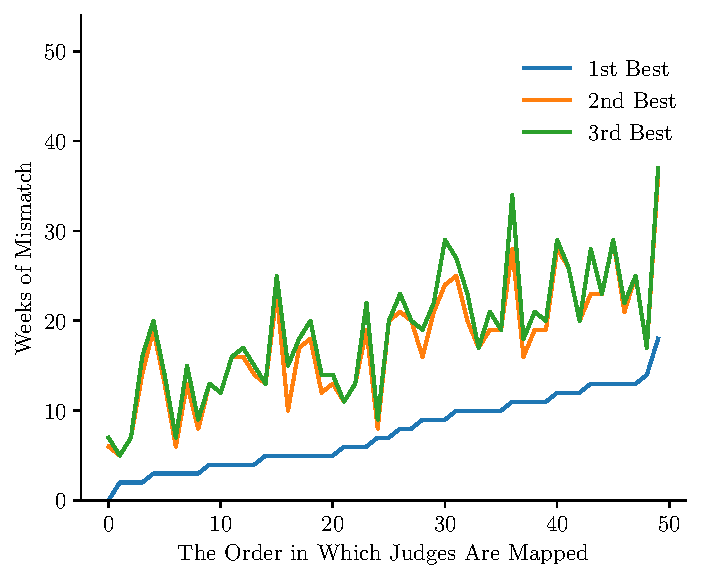
\includegraphics[scale=0.7]{Figures/First_Vs_Second_Vs_Third_Best_Match_Perfect}\label{Figure_Mapping_Mismatches_Perfect}}
    	\subfloat[{\small Overlapping Match.}]{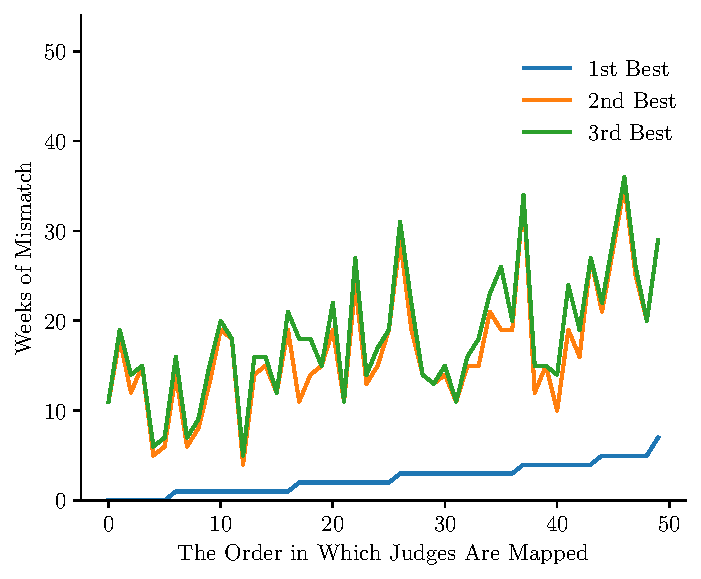
\includegraphics[scale=0.7]{Figures/First_Vs_Second_Vs_Third_Best_Match_Overlapping}\label{Figure_Mapping_Mismatches_Overlapping}}
    	\caption{Weeks of mismatch for the judge name mapped to each judge number. The judge names with the second and third fewest weeks of mismatch are also depicted.}
    	\label{Figure_Mapping_Mismatches}
    \end{figure}

  \subsection{Evaluating the mapping}
  	Next, we assess the performance of the (derived) mapping (from the judge numbers to the judge names). Under this mapping, we observe that only in $4.1\%$ of the sentencing events with a date, the judge was sentencing in a county to which he was not assigned. These $4.1\%$ problematic sentencing events belong to one of two categories: About $0.9\%$ belong to judge-week combinations in which the judge did not have any county assignments on the master calendar. The remaining $3.2\%$ belong to judge-week combinations in which the judge had county assignments on the master calendar. However, he was not assigned to the county in which the sentencing event occurred. Figure \ref{Figure_Mapping_Problematic_Sentencing_Events_Judge_Distribution} depicts the number of problematic sentencing events for each judge number. Figure \ref{Figure_Mapping_Problematic_Sentencing_Events_Week_Distribution} (in Appendix \ref{Sec:Appendix:Supplementary_Figures}) depicts the number of problematic sentencing events for each week. Figures \ref{Figure_Mapping_Problematic_Sentencing_Events_Judge_Distribution}-\ref{Figure_Mapping_Problematic_Sentencing_Events_Week_Distribution} show that the problematic sentencing events are not concentrated in just some judges or some weeks. These problematic sentencing events are discussed in detail in Section \ref{Sec:Master_Calendar:Further_Analysis_of_Some_Assignments}.

  \subsection{Limitations}
  	Assumption \ref{Assumption_Mapping_Only_County_Assignment_Matter} ignores the "circuit" assignments on the master calendar. Each circuit contains multiple counties. Instead, our matching algorithm works with the most granular geographic unit of interest, the county. As mentioned above, 3.2\% of the sentencing events with dates are at odds with the master calendar under the alphabetical mapping depicted in Table \ref{Table_Mapping_Judge_Numbers_To_Judge_Names}. Including "circuit" assignments and matching them on the basis of circuit courts as opposed to counties addresses only 12\% of the problematic sentencing events (corresponding to $0.4\%$ of the total number of sentencing events). As such, we stick with the choice of county for the matching purposes because it is more granular, and likely more accurate. Other assignments we ignore should be harmless because judges would not be involved in sentencing events or trials in those cases; see Figure  \ref{Figure_Assignment_Histogram}.

  	In addition, we focus only on the county names as opposed to the county name and the type of the assignment, which may also be listed; see Figure \ref{Figure_Assignment_Type_Histogram}. For example, Georgetown GS and Georgetown CP are both taken as Georgetown. There are several reasons for this: First, the type of the assignment is not always available. More importantly, all sentencing events should happen only in the general sessions (GS); and the common plea (CP) designation could be an error if a sentencing event appears in the sentencing dataset for the corresponding judge-week-county triple. Moreover, if no sentencing event occurs, then it is harmless to omit the CP designation. Consequently, focusing on the county name only makes the match easier.

  	Table \ref{Table_Schedule_Of_Unmapped_Judge_Names} (in Appendix \ref{Sec:Appendix:Supplementary_Figures}) depicts the list of counties visited by the fictitious judge (Juge 1) alongside the list of counties to which the unmapped judge names were assigned. Table \ref{Table_Schedule_Of_Unmapped_Judge_Names} shows that judge 1 is not a combination of the unmapped judge names.

% \section{Sample Selection for Service Rate Estimation}
%   \subsection{Sample Selection for estimation of $\theta$}
%     Our estimation procedure for $\mu_t$ relies on the assumption that judges only work on pleas or trials, and that they never idle. This is likely not true in general, so in order to estimate $\mu_t$, we have to identify the days in which it was likely that this held. We shall refer to these days as 'criminal days'. As mentioned in the data section, the calendar data includes information regarding the type of work the judge is expected to do in each assignment. We use this information to determine the days in which it is likely that a judge worked only on pleas or trials.
%     There are many different work types, and they are summarized below:
%     \begin{table}[H]
%       \centering
%       \caption{Assignment Type Acronyms}
%       \begin{tabular}{L{20mm}L{50mm}L{20mm}}
  \hline
  Acronym & Meaning & Share \\
  \hline
  %\rowgroup{Consumer Surplus} \\
  GS & General Session & 0.36 \\
  CC & Circuit Court & 0.02\\
  SGJ & State Grand Jury & 0.01\\
  CP & Common Pleas & 0.26 \\
  CPNJ & Common Pleas Non-Jury & 0.13 \\
  PCR & Post Conviction Relief & 0.03  \\
  Capital PCR & Capital Post Conviction Relief & < 0.01 \\
  AW & Administrative Week & 0.01 \\
  \hline
\end{tabular}

%     \end{table}
%
%     \paragraph{Days in which we observe sentencing events}
%       In theory, the only work type in which a judge can be reasonably expected to work exclusively on pleas and trials is GS. Furthermore, there are certain work types in which a judge shouldn't work on criminal cases, but we nevertheless observe criminal sentencing events. For example, the work type CP (common pleas) is for civil cases, but there are many sentencing events on CP days. This could be due to last minute changes that were not reflected in the calendar, or because the additional 'GS' acronym was omitted. To have a better sense of what days to include, we looked at the average number of pleas processed per day by each work type, conditional on observing a sentencing event on that day (see Figure \ref{fig-cond-avg}).
%       \begin{figure}[H]
%           \centering
%           \caption{Snapshot of Judge Calendar}
%           \label{fig-cond-avg}
%           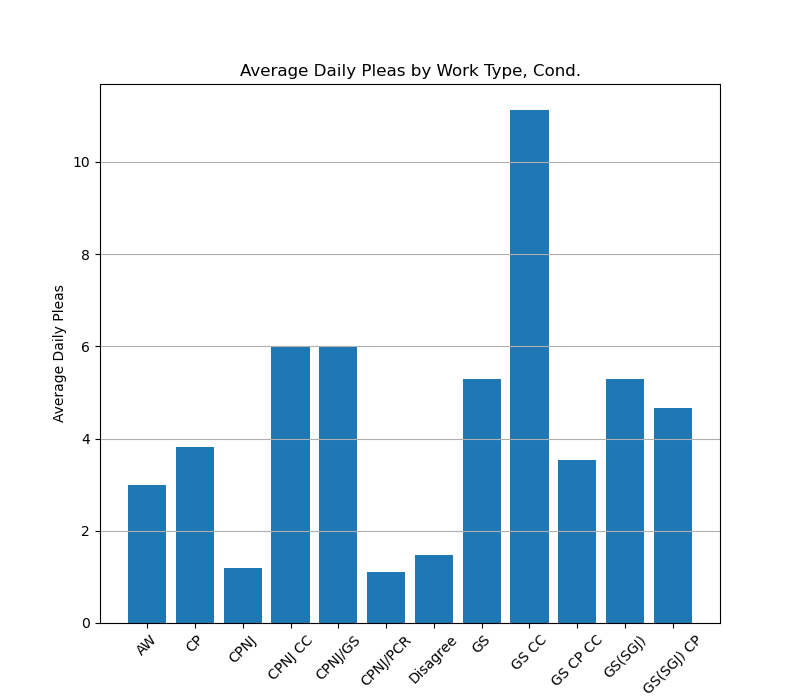
\includegraphics[width=0.75\textwidth, keepaspectratio=true]{../../output/figures/Exploration/avg_pleas_by_worktype_cond.png}
%         \end{figure}
%
%       Note that some work types (e.g. GS CC) are fairly uncommon, and are more influenced by outliers. As can be seen from the figure, if we condition on observing a sentencing event, then most of the different work types have roughly similar numbers of pleas processed per day (between 4 and 6). The exceptions to this are CPNJ, CPNJ/PCR, and times where there is a conflict between the sentencing data and the calendar data.
%
%     \paragraph{Days in which we don't observe sentencing events}
%       For each assignment type, there are many days in which we don't observe any sentencing events. The next question we had to resolve was which of these days to include. To get a better sense of this, we looked at the average number of pleas processed per day for each work type. Note that this differs from the quantities computed in the previous section because these are not conditional on observing a sentencing event. In other words, this calculation includes days in which we don't observe any sentencing events.
%
%       \begin{figure}[H]
%           \centering
%           \caption{Snapshot of Judge Calendar}
%           \label{fig-cond}
%           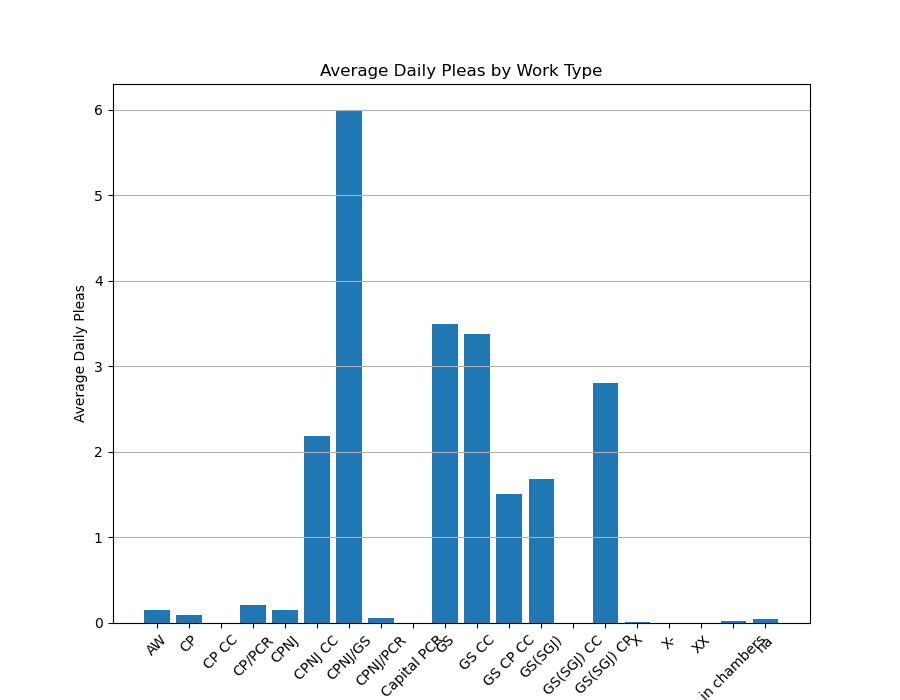
\includegraphics[width=0.75\textwidth, keepaspectratio=true]{../../output/figures/Exploration/avg_pleas_by_worktype.png}
%         \end{figure}
%
%       As can be seen from the figure, the average pleas processed per day drops considerably for many work types, especially those that do not include the GS work type. This suggests that for a majority of these days, the judges do not work on criminal cases, and that the days seen in the sentencing data are rare exceptions.
%
%       \paragraph{Decision}
%         As previously mentioned, our institutional knowledge suggests that we should count all GS days as criminal days. In addition to this, and following from the previous discussion, we decided to count any day in which we observe a sentencing event as a criminal day as well. For example, if there are 200 GS CC days and we observe sentencing events on 50 of them, we would count those 50 days as 'criminal days'. \textbf{Note/Proposal:} We could include non-GS, but weigh them by their productivity relative to GS days. So for example, if a day of type 'GS CC' sees half the pleas as a GS day, each 'GS CC' day would be counted as half a criminal day.
%
%     \paragraph{Sentencing events with missing dates}
%       As previously mentioned, some sentencing events have missing dates. However, they still have information regarding the county and the judge. As a result, we can use the calendar data to narrow down the set of dates in which the sentencing event could have happened. Here, we are assuming that we would only observe a sentencing event for judge $j$ in county $c$ on day $d$ if $j$ was scheduled to be in $c$ on $d$ according to the master calendar. So, for example, if judge 1 has 1 event with a missing date in Aiken county, and he was only assigned to Aiken county on two days according to the master calendar, then the sentencing event must have happened on one of those two days.
%
%       We will deal with trials with missing dates by assigning them as evenly as possible over the days in which the judge was assigned to that county. Suppose judge $j$ has $m$ sentencing events with missing dates in county $c$. We first use the calendar data to determine what days judge $j$ was scheduled to be in county $c$. Let $n_{jc}$ be the number of days that judge $j$ was scheduled to be in county $c$ and let $D_{jc}$ be the set of all days in which judge $j$ was scheduled to be in county $c$. We would assign the missing events to days as evenly as possible, and then assign the remaining days randomly. So, for example, if judge $j$ has 5 events with missing dates in county $c$ and was only scheduled to be in $c$ on two days, then both of those days would get 2 events, and the remaining event would be assigned randomly to one of those two days. \textbf{Question:} Will the set of possible days be those where we already observed sentencing events? Or will it be any day in which the judge was scheduled to be in the county? \textbf{Note:} I think it might be a good idea to restrict $D_{jc}$ and $n_{jc}$ to be the set/number of days in which the judge processed at least one sentencing event, otherwise, we will probably end up with a lot of days with just $1/n_{jc}$ pleas sentenced, which would be excluded from our capacity calculations because we currently exclude days with less than 1 sentencing event. However, this would assume that if a plea is processed at all, it is more likely that it was processed on a day in which other pleas were also processed. We should probably try both ways.
%
%   \subsection{Sample Selection for estimation of $\mu_t$}

\end{document}
